% ============================================================
%  Hybrid Cyber Attack Prediction Platform -- Group 14, CEK
%  B.Tech Final-Year Project Review -- Complete Technical Presentation
%  Synthesizing: EdgeFence (IJIS 2026), MGDA (Comput Netw 2026), Commander (JISA 2025)
%  Primary Benchmark: DARPA Transparent Computing (TC E3/E5)
%  Compile: pdflatex main.tex  (run twice for cross-references)
% ============================================================
\documentclass[aspectratio=169,10pt]{beamer}
\usetheme{Madrid}
\usecolortheme{default}
\usefonttheme{professionalfonts}
\usepackage[T1]{fontenc}
\usepackage{lmodern}
\usepackage{amsmath,amssymb}
\usepackage{booktabs}
\usepackage{tikz}
\usepackage{tabularx}
\usepackage{colortbl}
\usepackage{ragged2e}
\usepackage{array}
\usepackage{multirow}
\usetikzlibrary{arrows.meta,positioning,fit,backgrounds,calc,shadows,shapes.geometric}

% ---- TABLE COLUMN TYPES -----------------------------------------------
\newcolumntype{L}[1]{>{\raggedright\arraybackslash}p{#1}}
\newcolumntype{C}[1]{>{\centering\arraybackslash}p{#1}}
\newcolumntype{R}[1]{>{\raggedleft\arraybackslash}p{#1}}
\newcolumntype{Y}{>{\raggedright\arraybackslash}X}

% ---- COLOUR PALETTE ---------------------------------------------------
\definecolor{prismNavy}{RGB}{13,29,54}
\definecolor{prismBlue}{RGB}{38,126,190}
\definecolor{prismTeal}{RGB}{28,161,157}
\definecolor{prismMint}{RGB}{224,247,242}
\definecolor{prismGold}{RGB}{229,166,50}
\definecolor{rowA}{RGB}{240,248,255}
\definecolor{rowB}{RGB}{255,255,255}
\definecolor{strengthGreen}{RGB}{0,120,60}
\definecolor{limitRed}{RGB}{180,0,0}
\definecolor{codeBg}{RGB}{245,247,250}

% ---- BEAMER COLOURS ---------------------------------------------------
\setbeamercolor{structure}{fg=prismBlue}
\setbeamercolor{frametitle}{bg=prismNavy,fg=white}
\setbeamercolor{block title}{bg=prismBlue,fg=white}
\setbeamercolor{block body}{bg=prismMint,fg=black}
\setbeamertemplate{navigation symbols}{}
\setbeamercolor{author in head/foot}{bg=prismNavy,fg=white}
\setbeamercolor{title in head/foot}{bg=prismBlue,fg=white}
\setbeamercolor{date in head/foot}{bg=prismNavy,fg=white}
\setbeamertemplate{itemize item}{\color{prismTeal}$\blacktriangleright$}
\setbeamertemplate{itemize subitem}{\color{prismBlue}$\triangleright$}
\setbeamersize{text margin left=0.45cm,text margin right=0.45cm}

% ---- FOOTLINE ---------------------------------------------------------
\setbeamertemplate{footline}{%
  \leavevmode\hbox{%
  \begin{beamercolorbox}[wd=.333333\paperwidth,ht=2.25ex,dp=1ex,center]{author in head/foot}%
    \usebeamerfont{author in head/foot}Group 14 (CEK)\end{beamercolorbox}%
  \begin{beamercolorbox}[wd=.333333\paperwidth,ht=2.25ex,dp=1ex,center]{title in head/foot}%
    \usebeamerfont{title in head/foot}B.Tech Final-Year Project Review\end{beamercolorbox}%
  \begin{beamercolorbox}[wd=.333333\paperwidth,ht=2.25ex,dp=1ex,right]{date in head/foot}%
    \usebeamerfont{date in head/foot}\insertdate\hspace*{2em}\insertframenumber{}/\inserttotalframenumber\hspace*{2ex}\end{beamercolorbox}}%
  \vskip0pt}

% ---- FRAMETITLE -------------------------------------------------------
\setbeamertemplate{frametitle}{%
  \nointerlineskip%
  \begin{beamercolorbox}[wd=\paperwidth,ht=1.20cm,dp=0pt,leftskip=0.45cm,rightskip=0.45cm]{frametitle}%
    \vbox to 1.20cm{%
      \vfill%
      \raggedright\fontsize{9.2pt}{11.0pt}\selectfont\textbf{\insertframetitle}%
      \vfill%
    }%
  \end{beamercolorbox}%
}

% ---- DOCUMENT METADATA ------------------------------------------------
\title[Cyber Attack Prediction Platform]{CYBER ATTACK PREDICTION PLATFORM USING SPATIO-TEMPORAL GRAPH NEURAL NETWORKS}
\subtitle{Enterprise-to-Edge Provenance Analytics, Multi-Phase Cross-Machine Tracing \& Federated Adversarial GNNs on DARPA TC Benchmark}
\author{Muhammed Nasih K P \and Sumayya Ershad \and Najmunniza N \and K.S.\ Mahadev}
\institute{Dept.\ of Computer Science \& Engineering, College of Engineering, Karunagappally}
\date{October 2026}

% ---- HELPER COMMANDS --------------------------------------------------
\newcommand{\lrhdr}{%
  \rowcolor{prismNavy}%
  {\scriptsize\textcolor{white}{\textbf{Citation}}} &
  {\scriptsize\textcolor{white}{\textbf{Summary}}} &
  {\scriptsize\textcolor{white}{\textbf{Advantages \& Disadvantages}}} \\}

\newcommand{\stag}[1]{{\color{strengthGreen}\textbf{$\oplus$}~#1}}
\newcommand{\ltag}[1]{{\color{limitRed}\textbf{$\ominus$}~#1}}

% ---- PREVENT HYPHENATION (NO SPLIT WORDS) -----------------------------
\hyphenpenalty=10000
\exhyphenpenalty=10000
\sloppy

\begin{document}

%% ======================================================================
%%  TITLE SLIDE
%% ======================================================================
\begin{frame}[plain]
\begin{tikzpicture}[remember picture,overlay]
  \node[rounded corners=4pt,fill=prismBlue,drop shadow={shadow xshift=2pt,shadow yshift=-2pt,opacity=.35},
        minimum width=15.4cm,minimum height=1.10cm]
        at ([yshift=-0.80cm]current page.north) {};
  \node[text=white,font=\fontsize{11}{13}\selectfont\bfseries,align=center]
        at ([yshift=-0.80cm]current page.north) {CYBER ATTACK PREDICTION PLATFORM\\[0.06cm]
        USING SPATIO-TEMPORAL GRAPH NEURAL NETWORKS};
  \fill[prismNavy] (current page.south west) rectangle ([yshift=.45cm]current page.south east);
  \fill[prismBlue] ([xshift=5.33cm]current page.south west)
                    rectangle ([xshift=10.66cm,yshift=.45cm]current page.south west);
  \node[anchor=center,text=white,font=\scriptsize]
        at ([xshift=2.66cm,yshift=.22cm]current page.south west) {Group 14 (CEK)};
  \node[anchor=center,text=white,font=\scriptsize]
        at ([xshift=8cm,yshift=.22cm]current page.south west) {B.Tech Final-Year Project Review};
  \node[anchor=center,text=white,font=\scriptsize]
        at ([xshift=13.2cm,yshift=.22cm]current page.south west)
        {October 2026\hspace{1.2cm}1/\inserttotalframenumber};
  \node at ([yshift=6.80cm]current page.south)
        {
\includegraphics[height=1.10cm]{cek-logo.png}};
  \node[font=\footnotesize,align=center,text=prismNavy]
        at ([yshift=5.65cm]current page.south)
        {\textbf{Dept.\ of Computer Science \& Engineering}\\[.03cm]
         \textbf{College of Engineering, Karunagappally (CEK)}};
  \node[font=\small,align=center]
        at ([yshift=4.45cm]current page.south)
        {Under the Guidance of\\[.06cm]
         \textbf{\large Mrs.\ SYAMA S R}\\[.03cm]
         Assistant Professor, Dept.\ of CSE};
  \node[font=\large\bfseries,text=prismBlue]
        at ([yshift=3.35cm]current page.south) {Project Group 14};
  \node[font=\small]
        at ([yshift=1.80cm]current page.south)
        {\begin{tabular}{r@{\quad}l}
           \textbf{MUHAMMED NASIH K P} & \textbf{(KNP23CS074)} \\
           \textbf{SUMAYYA ERSHAD}     & \textbf{(KNP23CS107)} \\
           \textbf{NAJMUNNIZA N}       & \textbf{(LKNP20CS056)} \\
           \textbf{K.S.\ MAHADEV}      & \textbf{(KNP23CS066)}
         \end{tabular}};
\end{tikzpicture}
\end{frame}

%% ======================================================================
%%  PRESENTATION ROADMAP
%% ======================================================================
\begin{frame}{Presentation Overview}
\vspace{-0.2em}
\begin{columns}[T]
\begin{column}{0.48\textwidth}
\begin{beamercolorbox}[rounded=true,shadow=false,sep=0.35em,wd=\textwidth]{block title}
\textbf{\scriptsize Part I: Foundations, Review \& Core Methodology}
\end{beamercolorbox}
\vspace{0.20em}
{\fontsize{6.5pt}{8.3pt}\selectfont
\begin{itemize}\itemsep0.18em
  \item \textbf{Phase 1: Foundations \& Problem Formulation}
  \begin{itemize}\itemsep0.10em
    \item 1. Introduction \& Motivation
    \item 2. Problem Statement (SOC Challenges)
    \item 3. Objectives \& Target Milestones
    \item 4. Literature Review (16 Base Papers)
    \item 5. Research Gaps \& Proposed Solutions
  \end{itemize}
  \item \textbf{Phase 2: System Architecture \& Workflow}
  \begin{itemize}\itemsep0.10em
    \item 6. System Design Principles \& Benchmarks
    \item 7. End-to-End Workflow Diagram
  \end{itemize}
  \item \textbf{Phase 3: Multi-Model Detection Pipeline}
  \begin{itemize}\itemsep0.10em
    \item 8. Proposed Methods \& Formulations
    \item 9. Multi-Model Architecture \& Roles
    \item 10. End-to-End Inference Flow
  \end{itemize}
\end{itemize}
}
\end{column}
\begin{column}{0.48\textwidth}
\begin{beamercolorbox}[rounded=true,shadow=false,sep=0.35em,wd=\textwidth]{block title}
\textbf{\scriptsize Part II: Data, Schemas, Algorithms \& Management}
\end{beamercolorbox}
\vspace{0.20em}
{\fontsize{6.5pt}{8.3pt}\selectfont
\begin{itemize}\itemsep0.18em
  \item \textbf{Phase 4: Data Engineering \& Model Training}
  \begin{itemize}\itemsep0.10em
    \item 11. Dataset Preparation \& Loop Compaction
    \item 12. Model Training, Calibration \& Evaluation
  \end{itemize}
  \item \textbf{Phase 5: Deep Schemas \& Core Algorithms}
  \begin{itemize}\itemsep0.10em
    \item 13. System Architecture Diagram
    \item 14. Development \& Testing Flowchart
    \item 15. Dual-Tier Database Schemas
    \item 16. Core Algorithms \& Formal Pseudocode
  \end{itemize}
  \item \textbf{Phase 6: Implementation, Project Plan \& Conclusion}
  \begin{itemize}\itemsep0.10em
    \item 17. Implementation \& Technology Stack
    \item 18. Project Work Plan \& Gantt Roadmap
    \item 19. Conclusion \& Future Scope
    \item 20. References (Academic Literature)
  \end{itemize}
\end{itemize}
}
\end{column}
\end{columns}
\end{frame}

%%% ======================================================================
%%  1. INTRODUCTION
%% ======================================================================
\section{Introduction}

\begin{frame}{1. Introduction}
\vspace{0.6em}
\begin{beamercolorbox}[rounded=true,shadow=false,sep=0.80em,wd=\textwidth]{block body}
\fontsize{9.2pt}{14.5pt}\selectfont
Modern enterprise networks face hidden cyberattacks called \textbf{Advanced Persistent Threats (APTs)}, which avoid traditional security systems by behaving like normal users over long periods. Traditional intrusion detection systems often analyze logs separately, missing important connections between processes, files, and network connections (\textbf{Process} $\rightarrow$ \textbf{File} $\rightarrow$ \textbf{Socket}).

\vspace{0.4em}
Our system represents system activities as \textbf{dynamic provenance graphs} and combines \textbf{Graph Attention Networks (GAT)}, \textbf{Gated Recurrent Units (GRU)}, and \textbf{Variational Graph Autoencoders (VGAE)} to learn normal behavior and detect \textbf{unknown attacks without labeled training data}. It also uses \textbf{TenSEAL CKKS-encrypted Federated Learning} to enable secure collaboration between organizations while protecting their data.
\end{beamercolorbox}
\end{frame}

%% ======================================================================
%%  2. PROBLEM STATEMENT
%% ======================================================================
\section{Problem Statement}

\begin{frame}{2. Problem Statement}
\vspace{0.6em}
\begin{beamercolorbox}[rounded=true,shadow=false,sep=0.85em,wd=\textwidth]{block body}
\fontsize{9.3pt}{14.8pt}\selectfont
Traditional security systems struggle to detect \textbf{stealthy, multi-stage cyberattacks} because they \textbf{analyze system logs separately}, miss complex relationships and time-based attack patterns, and generate \textbf{false alarms} from normal activities. They also struggle to detect \textbf{unknown zero-day threats} while protecting sensitive data.

\vspace{0.4em}
This project proposes a \textbf{spatio-temporal graph-based anomaly detection framework} using \textbf{GAT}, \textbf{GRU}, and \textbf{VGAE} to detect suspicious activities, \textbf{reconstruct attack paths}, map threats to the \textbf{MITRE ATT\&CK framework}, and enable \textbf{privacy-preserving collaborative detection}.
\end{beamercolorbox}
\end{frame}

%% ======================================================================
%%  3. OBJECTIVES
%% ======================================================================
\section{Objectives}

\begin{frame}{3. Objectives}
\vspace{0.6em}
\begin{beamercolorbox}[rounded=true,shadow=false,sep=0.80em,wd=\textwidth]{block body}
\fontsize{9.2pt}{14.5pt}\selectfont
The main objective of this project is to develop an \textbf{intelligent and privacy-preserving cybersecurity system} that detects \textbf{hidden, multi-stage APT attacks} and \textbf{traces their attack paths} across enterprise networks.

\vspace{0.4em}
The system converts raw kernel audit logs from the \textbf{DARPA Transparent Computing dataset} into \textbf{provenance graphs} and uses \textbf{GAT, GRU, and VGAE} to \textbf{detect unknown attacks} by identifying unusual graph patterns. It also supports secure collaborative training using \textbf{TenSEAL CKKS encryption}, reconstructs attack paths across multiple computers, maps detected threats to the \textbf{MITRE ATT\&CK framework}, and displays the results on an \textbf{interactive SOC dashboard}.
\end{beamercolorbox}
\end{frame}

%% ======================================================================
%%  5. LITERATURE REVIEW (16 PAPERS - PRESERVED UNCHANGED)
%% ======================================================================
\section{Literature Review}

%% ------ P01 -----------------------------------------------------------
\begin{frame}[t]{MGDA: Provenance Graph Threat Detection \& Attack Scenario Reconstruction}
\vspace{-0.30em}
{\footnotesize\setlength{\tabcolsep}{3.5pt}\renewcommand{\arraystretch}{1.10}
\begin{tabularx}{\textwidth}{|L{3.10cm}|Y|L{5.70cm}|}
\hline\lrhdr\hline
\begin{minipage}[t]{\linewidth}\fontsize{7.2pt}{9.2pt}\raggedright\selectfont
\textbf{Author:}\par
Mengjiao Cui, Zhengwei Jiang, Shuai Li, Chunyan Ma, Kai Zhang, Peian Yang, and Huamin Feng\par\vspace{4pt}
\textbf{Year:} 2025\par\vspace{4pt}
\textbf{Journal:}\par
Computer Networks (Elsevier)\par\vspace{4pt}
\end{minipage}
&
\begin{minipage}[t]{\linewidth}\fontsize{7.2pt}{9.2pt}\raggedright\selectfont
Proposes \textbf{MGDA}, a self-supervised masked graph autoencoder on system provenance graphs for label-free APT detection. By learning normal behavior through masked node and edge reconstruction, anomalies are flagged via reconstruction errors, followed by causal tracing to reconstruct multi-stage attack scenarios.\par\vspace{4pt}
\end{minipage}
&
\begin{minipage}[t]{\linewidth}\fontsize{7.2pt}{9.0pt}\raggedright\selectfont
\textcolor{strengthGreen}{\textbf{Advantages:}}\par\vspace{1.5pt}
\textbullet~Detects unknown attacks without needing attack training labels.\par\vspace{2.0pt}\textbullet~Fast training in 14 minutes (100$\times$ speedup over baselines).\par\vspace{4.0pt}
\textcolor{limitRed}{\textbf{Disadvantages:}}\par\vspace{1.5pt}
\textbullet~Connects attack steps using manual rules rather than AI.\par\vspace{2.0pt}\textbullet~Inspects only event links, completely ignoring payload contents.\par\vspace{4pt}
\end{minipage} \\\hline
\end{tabularx}}
\end{frame}

%% ------ P02 -----------------------------------------------------------
\begin{frame}[t]{Commander: Robust Cross-Machine Multi-Phase APT Detection via Provenance}
\vspace{-0.30em}
{\footnotesize\setlength{\tabcolsep}{3.5pt}\renewcommand{\arraystretch}{1.10}
\begin{tabularx}{\textwidth}{|L{3.10cm}|Y|L{5.70cm}|}
\hline\lrhdr\hline
\begin{minipage}[t]{\linewidth}\fontsize{7.2pt}{9.2pt}\raggedright\selectfont
\textbf{Author:}\par
Qi Liu, Kaibin Bao, and Veit Hagenmeyer\par\vspace{4pt}
\textbf{Year:} 2025\par\vspace{4pt}
\textbf{Journal:}\par
Journal of Information Security and Applications (Elsevier)\par\vspace{4pt}
\end{minipage}
&
\begin{minipage}[t]{\linewidth}\fontsize{7.2pt}{9.2pt}\raggedright\selectfont
Proposes \textbf{Commander}, a cross-machine provenance analytics detector that tracks multi-phase APT lateral movement across distributed hosts. It uses logon-session partitioning to bound graph growth and prevent dependency explosion, correlating host audit logs with authentication events to trace attacker progression.\par\vspace{4pt}
\end{minipage}
&
\begin{minipage}[t]{\linewidth}\fontsize{7.2pt}{9.0pt}\raggedright\selectfont
\textcolor{strengthGreen}{\textbf{Advantages:}}\par\vspace{1.5pt}
\textbullet~Accurately tracks lateral attack movement across multiple hosts.\par\vspace{2.0pt}\textbullet~Session partitioning stops system graphs from growing too large.\par\vspace{4.0pt}
\textcolor{limitRed}{\textbf{Disadvantages:}}\par\vspace{1.5pt}
\textbullet~Strictly requires Windows Active Directory authentication logs.\par\vspace{2.0pt}\textbullet~Connecting attack paths across machines takes up to 9 minutes.\par\vspace{4pt}
\end{minipage} \\\hline
\end{tabularx}}
\end{frame}

%% ------ P03 -----------------------------------------------------------
\begin{frame}[t]{Threat Detection in CPS Through Spatio-Temporal Anomaly Detection Using GAT}
\vspace{-0.30em}
{\footnotesize\setlength{\tabcolsep}{3.5pt}\renewcommand{\arraystretch}{1.10}
\begin{tabularx}{\textwidth}{|L{3.10cm}|Y|L{5.70cm}|}
\hline\lrhdr\hline
\begin{minipage}[t]{\linewidth}\fontsize{7.2pt}{9.2pt}\raggedright\selectfont
\textbf{Author:}\par
Roberto Canonico, Francesco Lista, Annalisa Navarro, Giancarlo Sperl{\'\i}, and Andrea Vignali\par\vspace{4pt}
\textbf{Year:} 2025\par\vspace{4pt}
\textbf{Journal:}\par
Computers \& Security (Elsevier)\par\vspace{4pt}
\end{minipage}
&
\begin{minipage}[t]{\linewidth}\fontsize{7.2pt}{9.2pt}\raggedright\selectfont
Proposes an unsupervised spatio-temporal framework combining \textbf{Graph Attention Networks (GAT)} for spatial dependencies and recurrent units for temporal patterns. It detects complex cyber-physical anomalies from multivariate sensor streams via joint forecasting and reconstruction errors.\par\vspace{4pt}
\end{minipage}
&
\begin{minipage}[t]{\linewidth}\fontsize{7.2pt}{9.0pt}\raggedright\selectfont
\textcolor{strengthGreen}{\textbf{Advantages:}}\par\vspace{1.5pt}
\textbullet~Captures both sensor wiring links and rapid timing changes.\par\vspace{2.0pt}\textbullet~Fast 1.4-second detection enables quick real-time response.\par\vspace{4.0pt}
\textcolor{limitRed}{\textbf{Disadvantages:}}\par\vspace{1.5pt}
\textbullet~Assumes sensor topology stays fixed during operation.\par\vspace{2.0pt}\textbullet~Higher compute overhead compared to traditional baseline models.\par\vspace{4pt}
\end{minipage} \\\hline
\end{tabularx}}
\end{frame}

%% ------ P04 -----------------------------------------------------------
\begin{frame}[t]{EdgeFence: Federated Temporal GNNs for Adversarial Malware Detection in Edge Networks}
\vspace{-0.30em}
{\footnotesize\setlength{\tabcolsep}{3.5pt}\renewcommand{\arraystretch}{1.10}
\begin{tabularx}{\textwidth}{|L{3.10cm}|Y|L{5.70cm}|}
\hline\lrhdr\hline
\begin{minipage}[t]{\linewidth}\fontsize{7.2pt}{9.2pt}\raggedright\selectfont
\textbf{Author:}\par
Osei Isaac, Benjamin Appiah, Daniel Commey, Kwabena Owusu-Agyemang, Michael Asante, and Benjamin Hayfrom Acquah\par\vspace{4pt}
\textbf{Year:} 2026\par\vspace{4pt}
\textbf{Journal:}\par
International Journal of Information Security (Springer)\par\vspace{4pt}
\end{minipage}
&
\begin{minipage}[t]{\linewidth}\fontsize{7.2pt}{9.2pt}\raggedright\selectfont
Proposes \textbf{EdgeFence}, a federated learning framework for lightweight malware detection across distributed edge networks. Edge nodes model system call sequences as dynamic interaction graphs and locally train Temporal GNNs, sharing only model weights via FedAvg to preserve data privacy against adversarial threats.\par\vspace{4pt}
\end{minipage}
&
\begin{minipage}[t]{\linewidth}\fontsize{7.2pt}{9.0pt}\raggedright\selectfont
\textcolor{strengthGreen}{\textbf{Advantages:}}\par\vspace{1.5pt}
\textbullet~Keeps raw traffic on local devices to protect user privacy.\par\vspace{2.0pt}\textbullet~Temporal graph layers effectively catch evasive malware tricks.\par\vspace{4.0pt}
\textcolor{limitRed}{\textbf{Disadvantages:}}\par\vspace{1.5pt}
\textbullet~Differential privacy noise slightly lowers overall accuracy.\par\vspace{2.0pt}\textbullet~Constrained by mobile device battery and processing limits.\par\vspace{4pt}
\end{minipage} \\\hline
\end{tabularx}}
\end{frame}

%% ------ P05 -----------------------------------------------------------
\begin{frame}[t]{SHIELD: APT Detection and Intelligent Explanation Using Large Language Models}
\vspace{-0.30em}
{\footnotesize\setlength{\tabcolsep}{3.5pt}\renewcommand{\arraystretch}{1.10}
\begin{tabularx}{\textwidth}{|L{3.10cm}|Y|L{5.70cm}|}
\hline\lrhdr\hline
\begin{minipage}[t]{\linewidth}\fontsize{7.2pt}{9.2pt}\raggedright\selectfont
\textbf{Author:}\par
Parth Atulbhai Gandhi, Prasanna N. Wudali, Yonatan Amaru, Akansha Shukla, Yuval Elovici, and Asaf Shabtai\par\vspace{4pt}
\textbf{Year:} 2026\par\vspace{4pt}
\textbf{Journal:}\par
Engineering Applications of Artificial Intelligence (Elsevier)\par\vspace{4pt}
\end{minipage}
&
\begin{minipage}[t]{\linewidth}\fontsize{7.2pt}{9.2pt}\raggedright\selectfont
Proposes \textbf{SHIELD}, an end-to-end framework combining provenance graph anomaly detection with Large Language Models (LLMs). It isolates suspicious subgraphs from OS audit logs, prompting a fine-tuned LLM to verify attacks, generate plain-English explanations, and map activities to MITRE ATT\&CK techniques.\par\vspace{4pt}
\end{minipage}
&
\begin{minipage}[t]{\linewidth}\fontsize{7.1pt}{8.8pt}\raggedright\selectfont
\textcolor{strengthGreen}{\textbf{Advantages:}}\par\vspace{1.3pt}
\textbullet~Reduces false alarms and analyst workload.\par\vspace{1.8pt}\textbullet~Tracks slow-evolving attacks over long periods.\par\vspace{1.8pt}\textbullet~Provides clear and human-interpretable attack summaries.\par\vspace{3.2pt}
\textcolor{limitRed}{\textbf{Disadvantages:}}\par\vspace{1.3pt}
\textbullet~Requires high computational resources.\par\vspace{1.8pt}\textbullet~Can cause detection delay.\par\vspace{1.8pt}\textbullet~Depends on complete and accurate log capture.\par\vspace{3pt}
\end{minipage} \\\hline
\end{tabularx}}
\end{frame}

%% ------ P06 -----------------------------------------------------------
\begin{frame}[t]{From Logs to Tactics: Unsupervised APT Reconstruction with MITRE Meta-Alerts}
\vspace{-0.30em}
{\footnotesize\setlength{\tabcolsep}{3.5pt}\renewcommand{\arraystretch}{1.10}
\begin{tabularx}{\textwidth}{|L{3.10cm}|Y|L{5.70cm}|}
\hline\lrhdr\hline
\begin{minipage}[t]{\linewidth}\fontsize{7.2pt}{9.2pt}\raggedright\selectfont
\textbf{Author:}\par
Francesco Ferazza, Cosimo Melella, Konstantinos Mersinas, Ricardo Lugo, and Rain Ottis\par\vspace{4pt}
\textbf{Year:} 2026\par\vspace{4pt}
\textbf{Journal:}\par
International Journal of Information Security (Springer)\par\vspace{4pt}
\end{minipage}
&
\begin{minipage}[t]{\linewidth}\fontsize{7.2pt}{9.2pt}\raggedright\selectfont
Proposes an unsupervised framework that reconstructs full-scale APT campaigns from noisy audit logs. It uses Graph Autoencoders and Sentence-BERT to generate alert embeddings, clustering them into multi-stage attack sequences and achieving an 87\% F1-score in automated MITRE ATT\&CK mapping.\par\vspace{4pt}
\end{minipage}
&
\begin{minipage}[t]{\linewidth}\fontsize{6.8pt}{8.4pt}\raggedright\selectfont
\textcolor{strengthGreen}{\textbf{Advantages:}}\par\vspace{1.3pt}
\textbullet~Reduces alert overload by grouping many alerts into meaningful meta-alerts.\par\vspace{1.8pt}\textbullet~Works without labelled data using an unsupervised approach.\par\vspace{1.8pt}\textbullet~Handles noisy and heterogeneous logs from different sources.\par\vspace{3.2pt}
\textcolor{limitRed}{\textbf{Disadvantages:}}\par\vspace{1.3pt}
\textbullet~Depends on LLM summary quality, so incorrect summaries can affect later stages.\par\vspace{1.8pt}\textbullet~Ontology-based mapping can miss paraphrased expressions.\par\vspace{1.8pt}\textbullet~Evaluation was mainly based on exercise data, so broader real-world testing is needed.\par\vspace{3pt}
\end{minipage} \\\hline
\end{tabularx}}
\end{frame}

%% ------ P07 -----------------------------------------------------------
\begin{frame}[t]{A Novel Hybrid Intrusion Detection Method Integrating Anomaly and Misuse Detection}
\vspace{-0.30em}
{\footnotesize\setlength{\tabcolsep}{3.5pt}\renewcommand{\arraystretch}{1.10}
\begin{tabularx}{\textwidth}{|L{3.10cm}|Y|L{5.70cm}|}
\hline\lrhdr\hline
\begin{minipage}[t]{\linewidth}\fontsize{7.2pt}{9.2pt}\raggedright\selectfont
\textbf{Author:}\par
Gisung Kim, Seungmin Lee, and Sehun Kim\par\vspace{4pt}
\textbf{Year:} 2014\par\vspace{4pt}
\textbf{Journal:}\par
Expert Systems with Applications (Elsevier)\par\vspace{4pt}
\end{minipage}
&
\begin{minipage}[t]{\linewidth}\fontsize{7.2pt}{9.2pt}\raggedright\selectfont
Proposes a hierarchical dual-tier intrusion detection architecture integrating misuse and anomaly detection. A frontline Decision Tree rapidly filters known network attack signatures, while decomposed One-Class SVMs profile normal behavior to detect novel zero-day attacks with reduced overhead.\par\vspace{4pt}
\end{minipage}
&
\begin{minipage}[t]{\linewidth}\fontsize{6.8pt}{8.4pt}\raggedright\selectfont
\textcolor{strengthGreen}{\textbf{Advantages:}}\par\vspace{1.3pt}
\textbullet~Improves detection performance for both known and unknown attacks.\par\vspace{1.8pt}\textbullet~Reduces the training time of the anomaly detection model.\par\vspace{1.8pt}\textbullet~Uses known attack information to build more accurate normal-behavior profiles.\par\vspace{3.2pt}
\textcolor{limitRed}{\textbf{Disadvantages:}}\par\vspace{1.3pt}
\textbullet~C4.5 may split well-formed normal clusters.\par\vspace{1.8pt}\textbullet~Uneven data distribution reduces the expected reduction in training and testing time.\par\vspace{1.8pt}\textbullet~About 87\% of training data was concentrated in one subset, limiting the time-saving benefit.\par\vspace{3pt}
\end{minipage} \\\hline
\end{tabularx}}
\end{frame}

%% ------ P08 -----------------------------------------------------------
\begin{frame}[t]{Self-Supervised Graph Neural Networks for Network Intrusion Detection in Cloud-Edge}
\vspace{-0.30em}
{\footnotesize\setlength{\tabcolsep}{3.5pt}\renewcommand{\arraystretch}{1.10}
\begin{tabularx}{\textwidth}{|L{3.10cm}|Y|L{5.70cm}|}
\hline\lrhdr\hline
\begin{minipage}[t]{\linewidth}\fontsize{7.2pt}{9.2pt}\raggedright\selectfont
\textbf{Author:}\par
Haiyang Diao, Xiang Li, Wan Zhang, Yan Sibyl Yu, Ye Wang, and Jing Zhang\par\vspace{4pt}
\textbf{Year:} 2026\par\vspace{4pt}
\textbf{Journal:}\par
Journal of Cloud Computing (Springer)\par\vspace{4pt}
\end{minipage}
&
\begin{minipage}[t]{\linewidth}\fontsize{7.2pt}{9.2pt}\raggedright\selectfont
Proposes a self-supervised contrastive Graph Neural Network framework for network intrusion detection in cloud-edge environments. Modeling traffic flows as IP-port communication graphs, it learns robust topological representations from unlabeled traffic via multi-head attention without requiring labeled attack data.\par\vspace{4pt}
\end{minipage}
&
\begin{minipage}[t]{\linewidth}\fontsize{6.6pt}{8.1pt}\raggedright\selectfont
\textcolor{strengthGreen}{\textbf{Advantages:}}\par\vspace{1.3pt}
\textbullet~Reduces the dependency on labeled data by using self-supervised contrastive learning.\par\vspace{1.8pt}\textbullet~Captures both node and edge information using multi-head attention, which helps represent different malicious traffic patterns.\par\vspace{1.8pt}\textbullet~Reduces computational cost through dynamic attention-based edge pruning, which is useful for resource-constrained edge devices.\par\vspace{3.2pt}
\textcolor{limitRed}{\textbf{Disadvantages:}}\par\vspace{1.3pt}
\textbullet~High training computational overhead because Wasserstein and Gromov-Wasserstein distances are computationally expensive.\par\vspace{1.8pt}\textbullet~Sensitive to extreme class imbalance, causing poor detection of minority attack classes such as Theft and Backdoor.\par\vspace{1.8pt}\textbullet~Performance varies across datasets, with lower performance on complex datasets.\par\vspace{3pt}
\end{minipage} \\\hline
\end{tabularx}}
\end{frame}

%% ------ P09 -----------------------------------------------------------
\begin{frame}[t]{GraphShield: Advanced Dynamic Graph-Based Malware Detection Using GNNs}
\vspace{-0.30em}
{\footnotesize\setlength{\tabcolsep}{3.5pt}\renewcommand{\arraystretch}{1.10}
\begin{tabularx}{\textwidth}{|L{3.10cm}|Y|L{5.70cm}|}
\hline\lrhdr\hline
\begin{minipage}[t]{\linewidth}\fontsize{7.2pt}{9.2pt}\raggedright\selectfont
\textbf{Author:}\par
Eslam Amer, Shaker El-Sappagh, Tamer Abuhamad, Bander Ali Saleh Al-Rimy, and Alaa Mohasseb\par\vspace{4pt}
\textbf{Year:} 2025\par\vspace{4pt}
\textbf{Journal:}\par
Expert Systems with Applications (Elsevier)\par\vspace{4pt}
\end{minipage}
&
\begin{minipage}[t]{\linewidth}\fontsize{7.2pt}{9.2pt}\raggedright\selectfont
Proposes \textbf{GraphShield}, an explainable malware detection platform that converts dynamic program execution traces into behavioral interaction graphs. An attention-based GNN captures execution dependencies, while GNNExplainer highlights the exact malicious subgraphs to provide actionable explanations for analysts.\par\vspace{4pt}
\end{minipage}
&
\begin{minipage}[t]{\linewidth}\fontsize{7.2pt}{9.0pt}\raggedright\selectfont
\textcolor{strengthGreen}{\textbf{Advantages:}}\par\vspace{1.5pt}
\textbullet~Detects polymorphic malware by tracking behavioral graphs.\par\vspace{2.0pt}\textbullet~Outperforms static signature scanners on metamorphic variants.\par\vspace{4.0pt}
\textcolor{limitRed}{\textbf{Disadvantages:}}\par\vspace{1.5pt}
\textbullet~Requires sandbox execution to capture live malware behaviors.\par\vspace{2.0pt}\textbullet~Malware that delays actions or sleeps can evade detection.\par\vspace{4pt}
\end{minipage} \\\hline
\end{tabularx}}
\end{frame}

%% ------ P10 -----------------------------------------------------------
\begin{frame}[t]{Cyber Security Attack Recognition on Cloud Networks Based on GCN and GraphSAGE}
\vspace{-0.30em}
{\footnotesize\setlength{\tabcolsep}{3.5pt}\renewcommand{\arraystretch}{1.10}
\begin{tabularx}{\textwidth}{|L{3.10cm}|Y|L{5.70cm}|}
\hline\lrhdr\hline
\begin{minipage}[t]{\linewidth}\fontsize{7.2pt}{9.2pt}\raggedright\selectfont
\textbf{Author:}\par
Fargana Abdullayeva and Suleyman Suleymanzade\par\vspace{4pt}
\textbf{Year:} 2024\par\vspace{4pt}
\textbf{Journal:}\par
Results in Control and Optimization (Elsevier)\par\vspace{4pt}
\end{minipage}
&
\begin{minipage}[t]{\linewidth}\fontsize{7.2pt}{9.2pt}\raggedright\selectfont
Proposes modeling cloud network flows as communication graphs to classify multi-class attacks using GCN and GraphSAGE models. The inductive neighborhood sampling of GraphSAGE allows the model to generalize effectively to newly deployed virtual machines without full-graph retraining.\par\vspace{4pt}
\end{minipage}
&
\begin{minipage}[t]{\linewidth}\fontsize{7.2pt}{9.0pt}\raggedright\selectfont
\textcolor{strengthGreen}{\textbf{Advantages:}}\par\vspace{1.5pt}
\textbullet~Effectively captures communication topology between cloud instances.\par\vspace{2.0pt}\textbullet~GraphSAGE scales well to large, dynamic cloud networks.\par\vspace{4.0pt}
\textcolor{limitRed}{\textbf{Disadvantages:}}\par\vspace{1.5pt}
\textbullet~Tested on static offline logs rather than live cloud traffic.\par\vspace{2.0pt}\textbullet~Ignores internal host processes running inside virtual machines.\par\vspace{4pt}
\end{minipage} \\\hline
\end{tabularx}}
\end{frame}

%% ------ P11 -----------------------------------------------------------
\begin{frame}[t]{FTG-Net-E: Hierarchical Ensemble Graph Neural Network for DDoS Attack Detection}
\vspace{-0.30em}
{\footnotesize\setlength{\tabcolsep}{3.5pt}\renewcommand{\arraystretch}{1.10}
\begin{tabularx}{\textwidth}{|L{3.10cm}|Y|L{5.70cm}|}
\hline\lrhdr\hline
\begin{minipage}[t]{\linewidth}\fontsize{7.2pt}{9.2pt}\raggedright\selectfont
\textbf{Author:}\par
Rana Abu Bakar, Lorenzo De Marinis, Filippo Cugini, and Francesco Paolucci\par\vspace{4pt}
\textbf{Year:} 2024\par\vspace{4pt}
\textbf{Journal:}\par
Computer Networks (Elsevier)\par\vspace{4pt}
\end{minipage}
&
\begin{minipage}[t]{\linewidth}\fontsize{7.2pt}{9.2pt}\raggedright\selectfont
Proposes \textbf{FTG-Net-E}, a hierarchical ensemble Graph Neural Network for detecting high-volume DDoS floods and volumetric network attacks. By converting traffic into Flow Traffic Graphs (FTG), a two-level ensemble processes local and global traffic topology, achieving 99.2\% detection precision.\par\vspace{4pt}
\end{minipage}
&
\begin{minipage}[t]{\linewidth}\fontsize{7.2pt}{9.0pt}\raggedright\selectfont
\textcolor{strengthGreen}{\textbf{Advantages:}}\par\vspace{1.5pt}
\textbullet~Two-tier design filters massive floods with sub-millisecond delay.\par\vspace{2.0pt}\textbullet~Hierarchical ensemble minimizes false alarms during burst traffic.\par\vspace{4.0pt}
\textcolor{limitRed}{\textbf{Disadvantages:}}\par\vspace{1.5pt}
\textbullet~Specializes in high-rate DDoS and misses low-and-slow APTs.\par\vspace{2.0pt}\textbullet~Requires hardware acceleration (GPU/FPGA) to maintain wire speed.\par\vspace{4pt}
\end{minipage} \\\hline
\end{tabularx}}
\end{frame}

%% ------ P12 -----------------------------------------------------------
\begin{frame}[t]{Intelligent Intrusion Detection for Cyber-Physical Systems Using GAN-LSTM}
\vspace{-0.30em}
{\footnotesize\setlength{\tabcolsep}{3.5pt}\renewcommand{\arraystretch}{1.10}
\begin{tabularx}{\textwidth}{|L{3.10cm}|Y|L{5.70cm}|}
\hline\lrhdr\hline
\begin{minipage}[t]{\linewidth}\fontsize{7.2pt}{9.2pt}\raggedright\selectfont
\textbf{Author:}\par
Md Shakil Siddique, Md. Ashikur Rahman Khan, Ishtiaq Ahammad, Nishu Nath, Joysri Rani Das, and Fardowsi Rahman\par\vspace{4pt}
\textbf{Year:} 2025\par\vspace{4pt}
\textbf{Journal:}\par
Franklin Open (Elsevier)\par\vspace{4pt}
\end{minipage}
&
\begin{minipage}[t]{\linewidth}\fontsize{7.2pt}{9.2pt}\raggedright\selectfont
Proposes an intrusion detection framework for cyber-physical systems combining Generative Adversarial Networks (GAN) and LSTM networks. The GAN synthesizes realistic minority-class attack samples to overcome severe data imbalance, while the LSTM captures sequential temporal patterns in industrial telemetry logs.\par\vspace{4pt}
\end{minipage}
&
\begin{minipage}[t]{\linewidth}\fontsize{7.2pt}{9.0pt}\raggedright\selectfont
\textcolor{strengthGreen}{\textbf{Advantages:}}\par\vspace{1.5pt}
\textbullet~Solves the rare-attack data shortage using synthetic samples.\par\vspace{2.0pt}\textbullet~Successfully improves detection recall for rare intrusions by 28\%.\par\vspace{4.0pt}
\textcolor{limitRed}{\textbf{Disadvantages:}}\par\vspace{1.5pt}
\textbullet~GAN training can become unstable or generate unrealistic sensor values.\par\vspace{2.0pt}\textbullet~Analyzes sensor streams as parallel lines without graph topology.\par\vspace{4pt}
\end{minipage} \\\hline
\end{tabularx}}
\end{frame}

%% ------ P13 -----------------------------------------------------------
\begin{frame}[t]{Knowledge Graph Visualization and Anomaly Detection Using Graph Neural Networks}
\vspace{-0.30em}
{\footnotesize\setlength{\tabcolsep}{3.5pt}\renewcommand{\arraystretch}{1.10}
\begin{tabularx}{\textwidth}{|L{3.10cm}|Y|L{5.70cm}|}
\hline\lrhdr\hline
\begin{minipage}[t]{\linewidth}\fontsize{7.2pt}{9.2pt}\raggedright\selectfont
\textbf{Author:}\par
Ali Yilmaz, Resul Das, Mehmet Ozdem, and Berk Canberk\par\vspace{4pt}
\textbf{Year:} 2026\par\vspace{4pt}
\textbf{Journal:}\par
Computer Networks (Elsevier)\par\vspace{4pt}
\end{minipage}
&
\begin{minipage}[t]{\linewidth}\fontsize{7.1pt}{9.1pt}\raggedright\selectfont
Represents network communication as a graph, where IP addresses are nodes and communication flows are edges. Applies GCN, GAT, GIN, and GraphSAGE to detect network anomalies and identify suspicious communication patterns. Provides dynamic attack-topology visualization, helping security analysts understand relationships between network entities and possible attack paths.\par\vspace{4pt}
\end{minipage}
&
\begin{minipage}[t]{\linewidth}\fontsize{6.8pt}{8.4pt}\raggedright\selectfont
\textcolor{strengthGreen}{\textbf{Advantages:}}\par\vspace{1.3pt}
\textbullet~Represents communication between IPs as a graph, making attack connections easier to identify.\par\vspace{1.8pt}\textbullet~GNN models such as GIN and GraphSAGE achieved strong F1 and ROC-AUC results.\par\vspace{1.8pt}\textbullet~Provides attack-topology visualization to help analysts understand attacker--target relationships.\par\vspace{3.2pt}
\textcolor{limitRed}{\textbf{Disadvantages:}}\par\vspace{1.3pt}
\textbullet~Mainly focuses on network-level graph analysis, not live OS-level provenance.\par\vspace{1.8pt}\textbullet~Does not fully address temporal/dynamic graph behaviour.\par\vspace{1.8pt}\textbullet~Streaming graph updates and low-latency deployment need further development.\par\vspace{3pt}
\end{minipage} \\\hline
\end{tabularx}}
\end{frame}

%% ------ P14 -----------------------------------------------------------
\begin{frame}[t]{Robust, Efficient Detection of Network Intrusion Attacks: A Large Language Model Approach}
\vspace{-0.30em}
{\footnotesize\setlength{\tabcolsep}{3.5pt}\renewcommand{\arraystretch}{1.10}
\begin{tabularx}{\textwidth}{|L{3.10cm}|Y|L{5.70cm}|}
\hline\lrhdr\hline
\begin{minipage}[t]{\linewidth}\fontsize{7.2pt}{9.2pt}\raggedright\selectfont
\textbf{Author:}\par
Giancarlo Iannizzotto, Andrea Nucita, and Andrea Siragusa\par\vspace{4pt}
\textbf{Year:} 2026\par\vspace{4pt}
\textbf{Journal:}\par
Computer Networks (Elsevier)\par\vspace{4pt}
\end{minipage}
&
\begin{minipage}[t]{\linewidth}\fontsize{7.2pt}{9.2pt}\raggedright\selectfont
Proposes using fine-tuned open-source LLMs (LLaMA-3, Mistral) for contextual network intrusion detection. By serializing tabular flow records into structured text prompts, the language model captures subtle contextual relationships between flow features, demonstrating high resilience against adversarial perturbations.\par\vspace{4pt}
\end{minipage}
&
\begin{minipage}[t]{\linewidth}\fontsize{7.2pt}{9.0pt}\raggedright\selectfont
\textcolor{strengthGreen}{\textbf{Advantages:}}\par\vspace{1.5pt}
\textbullet~Pre-trained knowledge allows high detection without extensive task tuning.\par\vspace{2.0pt}\textbullet~Shows strong resilience against noisy or slightly altered attack flows.\par\vspace{4.0pt}
\textcolor{limitRed}{\textbf{Disadvantages:}}\par\vspace{1.5pt}
\textbullet~Token-by-token inference creates significant latency bottlenecks at wire speed.\par\vspace{2.0pt}\textbullet~Requires multi-GPU hardware servers to execute real-time inference.\par\vspace{4pt}
\end{minipage} \\\hline
\end{tabularx}}
\end{frame}

%% ------ P15 -----------------------------------------------------------
\begin{frame}[t]{Detection of Advanced Persistent Threat: A Genetic Programming Approach}
\vspace{-0.30em}
{\footnotesize\setlength{\tabcolsep}{3.5pt}\renewcommand{\arraystretch}{1.10}
\begin{tabularx}{\textwidth}{|L{3.10cm}|Y|L{5.70cm}|}
\hline\lrhdr\hline
\begin{minipage}[t]{\linewidth}\fontsize{7.2pt}{9.2pt}\raggedright\selectfont
\textbf{Author:}\par
Abdullah Al Mamun, Harith Al-Sahaf, Ian Welch, and Masood Mansoori\par\vspace{4pt}
\textbf{Year:} 2024\par\vspace{4pt}
\textbf{Journal:}\par
Applied Soft Computing (Elsevier)\par\vspace{4pt}
\end{minipage}
&
\begin{minipage}[t]{\linewidth}\fontsize{7.2pt}{9.2pt}\raggedright\selectfont
Proposes a Genetic Programming (GP) feature construction method for detecting multi-stage APT attacks in network traffic. Evolutionary algorithms automatically generate mathematical feature combinations from raw flow metrics, separating low-and-slow malicious connections from routine background traffic.\par\vspace{4pt}
\end{minipage}
&
\begin{minipage}[t]{\linewidth}\fontsize{7.2pt}{9.0pt}\raggedright\selectfont
\textcolor{strengthGreen}{\textbf{Advantages:}}\par\vspace{1.5pt}
\textbullet~Automatically discovers non-linear feature combinations without expert manual rules.\par\vspace{2.0pt}\textbullet~Evolved decision trees remain lightweight and interpretable for human inspection.\par\vspace{4.0pt}
\textcolor{limitRed}{\textbf{Disadvantages:}}\par\vspace{1.5pt}
\textbullet~Evolutionary search requires extensive multi-generation compute time.\par\vspace{2.0pt}\textbullet~Operates solely on static flow totals, missing host causal dependencies.\par\vspace{4pt}
\end{minipage} \\\hline
\end{tabularx}}
\end{frame}

%% ------ P16 -----------------------------------------------------------
\begin{frame}[t]{Dynamic Cyber Deception Using AI-Driven Adaptive Honeypot Networks}
\vspace{-0.30em}
{\footnotesize\setlength{\tabcolsep}{3.5pt}\renewcommand{\arraystretch}{1.10}
\begin{tabularx}{\textwidth}{|L{3.10cm}|Y|L{5.70cm}|}
\hline\lrhdr\hline
\begin{minipage}[t]{\linewidth}\fontsize{7.2pt}{9.2pt}\raggedright\selectfont
\textbf{Author:}\par
Mohammed Alshehri\par\vspace{4pt}
\textbf{Year:} 2026\par\vspace{4pt}
\textbf{Journal:}\par
Ain Shams Engineering Journal (Elsevier)\par\vspace{4pt}
\end{minipage}
&
\begin{minipage}[t]{\linewidth}\fontsize{7.2pt}{9.2pt}\raggedright\selectfont
Proposes an AI-driven dynamic cyber deception platform that deploys adaptive honeypot networks against multi-stage APT campaigns. Using reinforcement learning, it continuously reconfigures decoy services and synthetic vulnerabilities based on attacker probing, diverting adversaries and capturing high-fidelity telemetry.\par\vspace{4pt}
\end{minipage}
&
\begin{minipage}[t]{\linewidth}\fontsize{7.1pt}{8.8pt}\raggedright\selectfont
\textcolor{strengthGreen}{\textbf{Advantages:}}\par\vspace{1.3pt}
\textbullet~Dynamically changes honeypot behaviour according to attacker activity.\par\vspace{1.8pt}\textbullet~Makes deception more difficult for attackers to identify.\par\vspace{1.8pt}\textbullet~Records attacker activities and helps identify their tactics and techniques.\par\vspace{3.2pt}
\textcolor{limitRed}{\textbf{Disadvantages:}}\par\vspace{1.3pt}
\textbullet~Effectiveness depends on attackers interacting with the honeypot environment.\par\vspace{1.8pt}\textbullet~Continuous changes may cause over-reactive or unrealistic behaviour.\par\vspace{3pt}
\end{minipage} \\\hline
\end{tabularx}}
\end{frame}

%% ======================================================================
%% ======================================================================
%%  5. RESEARCH GAPS & PROPOSED SOLUTIONS (SINGLE SLIDE - TWO TABS)
%% ======================================================================
\section{Identified Research Gaps \& Proposed Solutions}

\begin{frame}[t]{5. Identified Research Gaps \& Proposed Solutions}
\vspace{-0.5em}
\begin{columns}[T]
%% ----------------------------------------------------------------------
%% Left Tab: Research Gaps
%% ----------------------------------------------------------------------
\begin{column}{0.485\textwidth}
\begin{beamercolorbox}[rounded=true,shadow=false,sep=0.32em,wd=\linewidth]{block title}
\textbf{\scriptsize \textcolor{limitRed}{\textbullet\ } Research Gaps (Existing Systems)}
\end{beamercolorbox}
\vspace{0.1em}
\begin{beamercolorbox}[rounded=true,shadow=false,sep=0.40em,wd=\linewidth]{block body}
{\fontsize{7.0pt}{9.6pt}\selectfont
\begin{itemize}\itemsep0.48em
  \item \textbf{1. Isolated Logs and Missed Attack Paths:}\\
  Existing tools analyze each computer separately, making it difficult to track attackers moving between machines. Combining all logs can also increase storage and processing costs.
  
  \item \textbf{2. Dependence on Known Attacks:}\\
  Many AI models require labeled attack data, making it difficult to detect new, unknown zero-day attacks and increasing false alarms.
  
  \item \textbf{3. Privacy Risks and High Resource Usage:}\\
  Sharing raw logs creates privacy risks, while complex graph AI models require too much time and computing power for resource-limited devices.
\end{itemize}
}
\end{beamercolorbox}
\end{column}

%% ----------------------------------------------------------------------
%% Right Tab: Proposed Solutions
%% ----------------------------------------------------------------------
\begin{column}{0.485\textwidth}
\begin{beamercolorbox}[rounded=true,shadow=false,sep=0.32em,wd=\linewidth]{block title}
\textbf{\scriptsize \textcolor{strengthGreen}{\textbullet\ } Proposed Solutions (Our System)}
\end{beamercolorbox}
\vspace{0.1em}
\begin{beamercolorbox}[rounded=true,shadow=false,sep=0.40em,wd=\linewidth]{block body}
{\fontsize{7.0pt}{9.6pt}\selectfont
\begin{itemize}\itemsep0.48em
  \item \textbf{1. Network-Wide Attack Tracking:}\\
  Connect related events across multiple computers to reconstruct complete attack paths while reducing unnecessary graph complexity.
  
  \item \textbf{2. Unsupervised Zero-Day Detection:}\\
  Use Masked-GAT to learn normal system behavior and identify unknown attacks without requiring labeled attack data.
  
  \item \textbf{3. Lightweight and Privacy-Preserving AI:}\\
  Run a compact model locally for fast detection and use TenSEAL CKKS-encrypted Federated Learning to train collaboratively without sharing raw system logs.
\end{itemize}
}
\end{beamercolorbox}
\end{column}
\end{columns}
\end{frame}

%% ======================================================================
%% ======================================================================
%%  6. SYSTEM DESIGN PRINCIPLES
%% ======================================================================
\section{System Design Principles}

\begin{frame}{6. System Design Principles: Core Features \& Architecture}
\vspace{0.2em}
\begin{beamercolorbox}[rounded=true,shadow=false,sep=0.38em,wd=\textwidth]{block title}
\textbf{\scriptsize 1. Core Architectural Pillars of AEGIS-PROV}
\end{beamercolorbox}
\vspace{0.15em}
{\fontsize{7.6pt}{10.8pt}\selectfont
\begin{itemize}\itemsep0.28em
  \item \textbf{Continuous Multi-OS Audit Ingestion:}\\
  Passively captures low-level operating system events in real time from Linux kernel audit hooks, Windows Sysmon, and industrial control streams, converting them into uniform graph records.
  \item \textbf{Semantics-Preserving Event Compaction:}\\
  Intelligently merges high-frequency repetitive operations (such as continuous file polling and socket reads), collapsing log volume by \textbf{$>85\%$} without losing any causal attack steps.
  \item \textbf{Decoupled Feature Representation:}\\
  Converts graph entities into lightweight 6D numeric vectors for microsecond GPU processing, while offloading long textual strings (file paths, hashes, IP addresses) into external lookup tables.
  \item \textbf{Dual-Tier AI Detection Engine:}\\
  Combines an on-device Edge-TGNN ($<80$~KB, 3.2~ms) for rapid local containment with an enterprise-level Masked-GAT autoencoder that learns normal behavior to catch unknown zero-day attacks.
  \item \textbf{Whole-Network Causal Tracing:}\\
  Uses logon-session boundaries and synthetic pseudo-edges to trace multi-stage lateral movement across Windows AD, Linux, and OT networks without overwhelming system memory.
\end{itemize}
}
\end{frame}

\begin{frame}{6. System Design Principles: Technologies \& Frameworks}
\vspace{0.2em}
\begin{beamercolorbox}[rounded=true,shadow=false,sep=0.38em,wd=\textwidth]{block title}
\textbf{\scriptsize 2. Technologies, Frameworks \& Core Libraries}
\end{beamercolorbox}
\vspace{0.2em}
{\fontsize{7.6pt}{11.0pt}\selectfont
\begin{itemize}\itemsep0.32em
  \item \textbf{Deep Learning \& Graph Frameworks:}\\
  Built with \textbf{Python 3.10+}, \textbf{PyTorch v2.2.0}, \textbf{PyTorch Geometric (PyG v2.5.0)}, and \textbf{DGL v1.1} for high-performance temporal graph modeling and spatial message passing.
  \item \textbf{Privacy-Preserving Federated Cryptography:}\\
  Utilizes \textbf{TenSEAL CKKS Homomorphic Encryption} for secure federated weight aggregation, allowing multiple organizations to train collaboratively without sharing raw logs or gradients.
  \item \textbf{High-Speed Ingestion \& Spatial Mathematics:}\\
  \textbf{FastAvro v1.9} for high-throughput binary CDM parsing, \textbf{SciPy v1.12} for high-dimensional K-d Tree spatial anomaly indexing ($k=10$), \textbf{NumPy}, and \textbf{Scikit-Learn}.
  \item \textbf{Kernel Sensors \& Probes:}\\
  \textbf{Linux Auditd}, \textbf{CamFlow v0.5} Linux Security Module (LSM) hooks, and \textbf{Windows Sysmon v14} with Windows Event Forwarding (WEF).
  \item \textbf{Forensic Dashboard \& Microservices:}\\
  Asynchronous \textbf{FastAPI} REST backend coupled with a \textbf{Cytoscape.js} interactive graph canvas for real-time SOC kill-chain investigation.
\end{itemize}
}
\end{frame}

\begin{frame}[t]{6. System Design Principles: Benchmark Dataset: DARPA TC}
\vspace{-0.2em}
\begin{beamercolorbox}[rounded=true,shadow=false,sep=0.35em,wd=\textwidth]{block title}
\textbf{\scriptsize 3. Benchmark Dataset: DARPA Transparent Computing (TC)}
\end{beamercolorbox}
\vspace{0.1em}
{\fontsize{7.2pt}{9.8pt}\selectfont
\begin{itemize}\itemsep0.18em
  \item \textbf{Gold Standard for APT Provenance Analytics:}\\
  The project exclusively utilizes the \textbf{DARPA Transparent Computing (TC) Engagement~3 (E3)} dataset, the authoritative benchmark for evaluating enterprise-wide provenance-based intrusion detection systems.
  \item \textbf{Subsets Evaluated (Real Multi-Stage Red-Team Attacks):}
    \begin{itemize}\itemsep0.10em
      \item \textbf{E3-CADETS (FreeBSD / OpenBSM):} 1.62M nodes, 3.30M edges. Evaluates detection of an Nginx memory corruption exploit, spawned shell, payload dropper (\texttt{/tmp/vUgefal}), and in-memory injection into \texttt{sshd}.
      \item \textbf{E3-THEIA (Linux Ubuntu / LSM):} 1.62M nodes, 2.87M edges. Evaluates defense against browser drive-by exploits, root privilege escalation, credential theft, and sensitive file exfiltration.
      \item \textbf{E3-TRACE (Linux Ubuntu / CamFlow \& Auditd):} 3.28M nodes, 4.08M edges. Continuous 2-week recording featuring a stealthy Firefox backdoor, cron persistence, and SSH lateral movement across machines.
    \end{itemize}
  \item \textbf{Why Exclusively DARPA TC? Ground-Truth Enterprise Provenance:}\\
  Contains authentic multi-stage cyber attacks executed by nation-state caliber red teams interleaved with dense benign background activity. It provides full kernel-level causal visibility across processes, files, and network sockets under a unified Common Data Model (CDM).
\end{itemize}
}
\end{frame}

\begin{frame}{6. System Design Principles: Dual-Tier Database Architecture}
\vspace{0.2em}
\begin{beamercolorbox}[rounded=true,shadow=false,sep=0.38em,wd=\textwidth]{block title}
\textbf{\scriptsize 4. Dual-Tier Database Architecture: Graph + Relational}
\end{beamercolorbox}
\vspace{0.2em}
{\fontsize{7.6pt}{11.0pt}\selectfont
\begin{itemize}\itemsep0.32em
  \item \textbf{Neo4j Enterprise 5.x (Graph Provenance Store):}\\
  Purpose-built for relationship traversal. Stores whole-system provenance DAGs with indexed node entities (\texttt{:Process}, \texttt{:File}, \texttt{:Socket}, \texttt{:Host}) and causal relationship edges (\texttt{[:FORK]}, \texttt{[:READ]}, \texttt{[:WRITE]}, \texttt{[:CONNECT]}, and synthetic pseudo-edges); native graph index pointers deliver sub-second multi-hop causal queries.
  \item \textbf{PostgreSQL 16 (Relational Metadata Store):}\\
  Guarantees ACID compliance for structured security records:
  \begin{itemize}\itemsep0.15em
    \item \texttt{hosts}: Tracks connected endpoint asset inventory, platform details, and health status.
    \item \texttt{anomalies}: Logs individual AI anomaly detection seeds, scores, and detector sources.
    \item \texttt{attack\_graphs}: Stores reconstructed multi-stage attack DAGs with MITRE ATT\&CK tags.
    \item \texttt{federated\_updates}: Records model weights, loss deltas, and training rounds.
  \end{itemize}
\end{itemize}
}
\end{frame}

%% ======================================================================
%%  7. WORKFLOW DIAGRAM
%% ======================================================================
\section{Workflow Diagram}

\begin{frame}{7. Workflow Diagram: End-to-End System Processing Pipeline}
\vspace{-0.15em}
\centering
\resizebox{0.98\textwidth}{!}{%
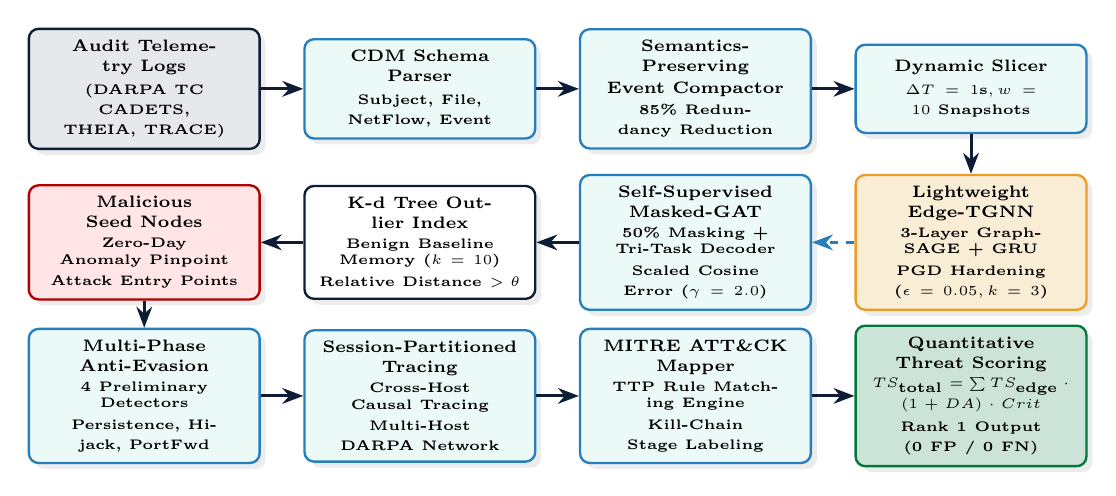
\begin{tikzpicture}[
  box/.style={draw=prismNavy, fill=white, rounded corners=3.5pt, line width=0.85pt,
              font=\fontsize{6.2}{7.2}\selectfont\bfseries, align=center, inner sep=4pt,
              text width=2.65cm, minimum height=1.12cm, drop shadow={opacity=0.15}},
  proc/.style={draw=prismBlue, fill=prismMint!60, rounded corners=3.5pt, line width=0.85pt,
               font=\fontsize{6.2}{7.2}\selectfont\bfseries, align=center, inner sep=4pt,
               text width=2.65cm, minimum height=1.12cm, drop shadow={opacity=0.15}},
  fl/.style={draw=prismGold!80!orange, fill=prismGold!20, rounded corners=3.5pt, line width=0.85pt,
             font=\fontsize{6.2}{7.2}\selectfont\bfseries, align=center, inner sep=4pt,
             text width=2.65cm, minimum height=1.12cm, drop shadow={opacity=0.15}},
  alert/.style={draw=limitRed, fill=red!10, rounded corners=3.5pt, line width=0.85pt,
                font=\fontsize{6.2}{7.2}\selectfont\bfseries, align=center, inner sep=4pt,
                text width=2.65cm, minimum height=1.12cm, drop shadow={opacity=0.15}},
  arrow/.style={-{Stealth[scale=0.95]}, line width=1.1pt, color=prismNavy},
  darrow/.style={-{Stealth[scale=0.95]}, line width=1.1pt, dashed, color=prismBlue}
]

% Row 1: Ingestion, Compaction & Slicing (Left to Right)
\node[box, fill=prismNavy!10] (raw) at (0, 0) {Audit Telemetry Logs\\[0.04cm]\tiny (DARPA TC CADETS, THEIA, TRACE)};
\node[proc] (parse) at (3.5, 0) {CDM Schema Parser\\[0.04cm]\tiny Subject, File, NetFlow, Event};
\node[proc] (comp) at (7.0, 0) {Semantics-Preserving\\[0.02cm]Event Compactor\\[0.02cm]\tiny 85\% Redundancy Reduction};
\node[proc] (slice) at (10.5, 0) {Dynamic Slicer\\[0.04cm]\tiny $\Delta T=1\text{s}, w=10$ Snapshots};

% Row 2: Detection Engines (Right to Left)
\node[fl] (edge) at (10.5, -1.95) {Lightweight Edge-TGNN\\[0.04cm]\tiny 3-Layer GraphSAGE + GRU\\[0.02cm]\tiny PGD Hardening ($\epsilon=0.05, k=3$)};
\node[proc] (gat) at (7.0, -1.95) {Self-Supervised Masked-GAT\\[0.04cm]\tiny 50\% Masking + Tri-Task Decoder\\[0.02cm]\tiny Scaled Cosine Error ($\gamma=2.0$)};
\node[box] (kdtree) at (3.5, -1.95) {K-d Tree Outlier Index\\[0.04cm]\tiny Benign Baseline Memory ($k=10$)\\[0.02cm]\tiny Relative Distance $> \theta$};
\node[alert] (seeds) at (0, -1.95) {Malicious Seed Nodes\\[0.04cm]\tiny Zero-Day Anomaly Pinpoint\\[0.02cm]\tiny Attack Entry Points};

% Row 3: Whole-Network Tracing & Attribution (Left to Right)
\node[proc] (cmd) at (0, -3.90) {Multi-Phase Anti-Evasion\\[0.04cm]\tiny 4 Preliminary Detectors\\[0.02cm]\tiny Persistence, Hijack, PortFwd};
\node[proc] (trace) at (3.5, -3.90) {Session-Partitioned Tracing\\[0.04cm]\tiny Cross-Host Causal Tracing\\[0.02cm]\tiny Multi-Host DARPA Network};
\node[proc] (mitre) at (7.0, -3.90) {MITRE ATT\&CK Mapper\\[0.04cm]\tiny TTP Rule Matching Engine\\[0.02cm]\tiny Kill-Chain Stage Labeling};
\node[box, fill=strengthGreen!20, draw=strengthGreen] (score) at (10.5, -3.90) {Quantitative Threat Scoring\\[0.04cm]\tiny $TS_{\text{total}} = \sum TS_{\text{edge}} \cdot (1+DA) \cdot Crit$\\[0.04cm]\tiny \textbf{Rank 1 Output (0 FP / 0 FN)}};

% Row 1 Connectors
\draw[arrow] (raw) -- (parse);
\draw[arrow] (parse) -- (comp);
\draw[arrow] (comp) -- (slice);

% Row 1 to Row 2: Pure Vertical Connector
\draw[arrow] (slice) -- (edge);

% Row 2 Connectors
\draw[darrow] (edge) -- (gat);
\draw[arrow] (gat) -- (kdtree);
\draw[arrow] (kdtree) -- (seeds);

% Row 2 to Row 3: Pure Vertical Connector
\draw[arrow] (seeds) -- (cmd);

% Row 3 Connectors
\draw[arrow] (cmd) -- (trace);
\draw[arrow] (trace) -- (mitre);
\draw[arrow] (mitre) -- (score);

\end{tikzpicture}}
\end{frame}

%% ======================================================================
%%  8. PROPOSED METHODS
%% ======================================================================
\section{Proposed Methods}

\begin{frame}[t]{8. Proposed Methods: Lightweight Edge-TGNN with Adversarial Defense}
\vspace{-0.25em}
\begin{beamercolorbox}[rounded=true,shadow=false,sep=0.30em,wd=\textwidth]{block title}
\textbf{\scriptsize 1. Lightweight Edge-TGNN with On-Device PGD Hardening (Edge Sentry)}
\end{beamercolorbox}
\vspace{0.08em}
{\fontsize{6.8pt}{9.2pt}\selectfont
\setlength{\abovedisplayskip}{1.5pt}
\setlength{\belowdisplayskip}{1.5pt}
\begin{itemize}\itemsep0.10em
  \item \textbf{Spatial GNN (3-Layer GraphSAGE Encoder):}\\
  Gathers causal context from immediate process-file-socket neighborhoods with hidden size $d_h=32$, ensuring an ultra-low memory footprint ($<1$~MB RAM):
  $$h_v^{(l)} = \text{ReLU}\left(W_{\text{self}}^{(l)} h_v^{(l-1)} + W_{\text{neigh}}^{(l)} \frac{1}{|N(v)|}\sum_{u \in N(v)} h_u^{(l-1)}\right)$$
  \item \textbf{Temporal Recurrence (Gated Recurrent Unit):}\\
  Captures multi-second temporal execution sequences across rolling snapshots ($\Delta T = 1\text{s}, w = 10, d_{\text{gru}}=64$):
  $$h_{i,t}^{\text{temp}} = \text{GRU}(h_{G_t}, h_{i,t-1}^{\text{temp}})$$
  \item \textbf{3-Step Continuous PGD Adversarial Hardening:}\\
  Simulates evasive attacker noise (dummy syscall injection, $k_{\text{mod}} \le 3, \epsilon=0.05$) directly on-device during training, hardening the model against evasion before deployment:
  $$\delta^* = \arg\max_{\|\delta\| \le \Omega} \ell(f_\theta(G+\delta), y)$$
  \item \textbf{Privacy-Preserving Federated Collaboration:}\\
  Transmits only 79.63~KB model parameter deltas $\Delta \theta_i$ protected by TenSEAL CKKS encryption; sensitive raw enterprise telemetry never leaves the endpoint.
\end{itemize}
}
\end{frame}

\begin{frame}{8. Proposed Methods: Self-Supervised Masked-GAT Autoencoder}
\vspace{0.15em}
\begin{beamercolorbox}[rounded=true,shadow=false,sep=0.38em,wd=\textwidth]{block title}
\textbf{\scriptsize 2. Self-Supervised Masked-GAT Autoencoder (Zero-Day Pinpointing)}
\end{beamercolorbox}
\vspace{0.15em}
{\fontsize{7.4pt}{10.6pt}\selectfont
\begin{itemize}\itemsep0.25em
  \item \textbf{50\% Stochastic Attribute Masking:}\\
  Hides half of the node features while preserving structural graph causality, forcing the model to deeply learn normal everyday system behavior without requiring labeled attack examples.
  \item \textbf{Multi-Layer Attention Message Passing:}\\
  Computes edge-type aware attention coefficients $\alpha_{nu}^{(l)}$ and concatenates multi-scale contextual representations across all layers: $H_n = h_n^{(1)} \parallel h_n^{(2)} \parallel h_n^{(3)}$.
  \item \textbf{Tri-Task Self-Supervised Decoder:}\\
  Optimizes three joint objectives simultaneously:
  \begin{itemize}\itemsep0.12em
    \item \textit{Task 1 (Feature Reconstruction)}: Scaled Cosine Error ($\gamma=2.0$) focusing on hard-to-predict anomalies.
    \item \textit{Task 2 (Latent Target Matching)}: Aligns corrupted representations with an exponential moving average target.
    \item \textit{Task 3 (Structure Link Prediction)}: Reconstructs causal edges via Binary Cross Entropy.
  \end{itemize}
  \item \textbf{High-Dimensional K-d Tree Outlier Scoring:}\\
  Compares test node representations against the 10 nearest normal neighbors in benign memory ($k=10$); nodes exceeding threshold $\theta=1.5$ are flagged as anomalous zero-day attack seeds $\mathcal{M}$.
\end{itemize}
}
\end{frame}

\begin{frame}{8. Proposed Methods: Cross-Machine Tracing Engine}
\vspace{0.15em}
\begin{beamercolorbox}[rounded=true,shadow=false,sep=0.38em,wd=\textwidth]{block title}
\textbf{\scriptsize 3. Session-Partitioned Cross-Machine Tracing Engine (Commander Core)}
\end{beamercolorbox}
\vspace{0.15em}
{\fontsize{7.4pt}{10.6pt}\selectfont
\begin{itemize}\itemsep0.25em
  \item \textbf{Logon-Session Boundary Graph Partitioning:}\\
  Naive graph traversal causes catastrophic \textit{dependency explosion}. By partitioning whole-system logs into user Logon Sessions ($L_{id}$), reachability is tightly bounded, preventing traversal bloat.
  \item \textbf{Synthetic Pseudo-Edge Resolution:}\\
  Disjoint attack steps separated by execution boundaries are bridged by synthetic links:
  \begin{itemize}\itemsep0.12em
    \item \textit{Persistence}: Links registry Run keys and scheduled task setups to their later trigger execution.
    \item \textit{Session Hijacking}: Links token duplication and elevation to new unauthorized logon sessions.
    \item \textit{Port Forwarding}: Remaps local proxy loopback sockets back to remote attacker command IPs.
  \end{itemize}
  \item \textbf{Enterprise Multi-Host Lateral Correlation:}\\
  Seamlessly follows lateral pivot chains across enterprise workstations and server endpoints (FreeBSD and Linux) within the DARPA multi-host network.
\end{itemize}
}
\end{frame}

\begin{frame}[t]{8. Proposed Methods: Quantitative Threat Scoring \& ATT\&CK Mapping}
\vspace{-0.25em}
\begin{beamercolorbox}[rounded=true,shadow=false,sep=0.30em,wd=\textwidth]{block title}
\textbf{\scriptsize 4. Quantitative ATT\&CK Threat Scoring \& Incident Prioritization}
\end{beamercolorbox}
\vspace{0.08em}
{\fontsize{6.8pt}{9.2pt}\selectfont
\setlength{\abovedisplayskip}{1.5pt}
\setlength{\belowdisplayskip}{1.5pt}
\begin{itemize}\itemsep0.10em
  \item \textbf{Edge Threat Score Formulation:}\\
  Every causal transition edge $e$ in the reconstructed attack graph is evaluated based on tactic severity and frequency:
  $$TS_{\text{edge}} = \sum_{i} w_i \cdot \left[ Freq(teq_i) + Var(tac_i) \right]$$
  where credential theft ($w=3.0$) and persistence ($w=2.5$) carry the highest weights.
  \item \textbf{Total Scenario Threat Score ($TS_{\text{total}}$):}\\
  Aggregates across all lateral movement edges with critical asset multipliers:
  $$TS_{\text{total}} = \sum TS_{\text{edge}} \cdot (1 + \mathbb{I}_{\text{DomainAdmin}}) \cdot \text{Criticality}_{\text{host}}$$
  \item \textbf{Rank-1 Incident Prioritization (Zero False Alarms):}\\
  Scores and sorts all candidate subgraphs, successfully surfacing the true multi-stage APT campaign at \textbf{Rank 1 (0 FP / 0 FN)} on the interactive SOC dashboard.
  \item \textbf{MITRE ATT\&CK Mapping:}\\
  Automatically maps every step of the reconstructed graph to official MITRE tactics (Initial Access $\to$ Execution $\to$ Persistence $\to$ Lateral Movement $\to$ Exfiltration).
\end{itemize}
}
\end{frame}

%% ======================================================================
%%  9. MODEL RESPONSIBILITIES AND INFERENCE FLOW
%% ======================================================================
\section{Model Responsibilities \& Inference Flow}

\begin{frame}{9. Model Responsibilities: Model 1 — Edge-TGNN (Perimeter Sentry)}
\vspace{0.15em}
\begin{beamercolorbox}[rounded=true,shadow=false,sep=0.35em,wd=\textwidth]{block title}
\textbf{\scriptsize Model 1: Lightweight Edge-TGNN (On-Device Perimeter Sentry)}
\end{beamercolorbox}
\vspace{0.15em}
{\fontsize{7.5pt}{10.5pt}\selectfont
\begin{itemize}\itemsep0.22em
  \item \textbf{Primary Operational Role:}\\
  First line of defense deployed on local edge nodes, IoT gateways, and endpoint agents for millisecond-level screening.
  \item \textbf{Input Data Stream:}\\
  Dynamic rolling temporal graph snapshots $\{G_{t-9}, \dots, G_t\}$ with slice duration $\Delta T = 1\text{s}$ and window $w = 10$.
  \item \textbf{Neural Architecture:}\\
  3-Layer GraphSAGE (mean aggregation, $d_h=32$) coupled to a 1-Layer GRU ($d_{\text{gru}}=64$) and global mean pooling readout.
  \item \textbf{Footprint \& Latency:}\\
  Ultra-compact 79.63~KB parameter footprint, requires $<1$~MB RAM, and executes inference in just \textbf{3.2~ms} per snapshot.
  \item \textbf{Adversarial Defense:}\\
  Hardened against structural evasion via an on-device 3-step continuous PGD loop ($\epsilon=0.05, k_{\text{mod}} \le 3$).
  \item \textbf{Detection Criterion \& Output:}\\
  Calculates local maliciousness probability score $s_{i,t} \in [0,1]$. Dispatches an immediate edge isolation alarm and triggers SOC escalation whenever $s_{i,t} \ge \tau_{\text{edge}}$.
\end{itemize}
}
\end{frame}

\begin{frame}{9. Model Responsibilities: Model 2 — Masked-GAT (SOC Deep Analyzer)}
\vspace{0.15em}
\begin{beamercolorbox}[rounded=true,shadow=false,sep=0.35em,wd=\textwidth]{block title}
\textbf{\scriptsize Model 2: Self-Supervised Masked-GAT Autoencoder (SOC Deep Analyzer)}
\end{beamercolorbox}
\vspace{0.15em}
{\fontsize{7.5pt}{10.5pt}\selectfont
\begin{itemize}\itemsep0.22em
  \item \textbf{Primary Operational Role:}\\
  Centralized enterprise analyzer running on GPU clusters to pinpoint zero-day process execution anomalies without labeled training data.
  \item \textbf{Input Data Stream:}\\
  Compacted whole-host provenance graphs generated from DARPA TC audit streams with repetitive loops collapsed ($>85\%$ compaction).
  \item \textbf{Neural Architecture:}\\
  Stacked multi-layer GAT encoder with edge-type attention and layer concatenation, paired with a Tri-Task decoder.
  \item \textbf{Self-Supervised Masking \& Loss:}\\
  Applies 50\% stochastic attribute masking. Optimized using Scaled Cosine Error ($\gamma=2.0$) to focus reconstruction on subtle anomalies.
  \item \textbf{Detection Criterion (Spatial Outlier Scoring):}\\
  Embeds reconstructed vectors into a benign memory indexed by a K-d tree ($k=10$). Process nodes with relative spatial distance $\frac{\bar{D}_{\text{test}}}{\bar{D}_{\text{train}}} > \theta$ ($\theta=1.5$) are flagged as anomalous seed processes $\mathcal{M}$.
\end{itemize}
}
\end{frame}

\begin{frame}{9. Model Responsibilities: Model 3 — Causal Tracing Engine}
\vspace{0.15em}
\begin{beamercolorbox}[rounded=true,shadow=false,sep=0.35em,wd=\textwidth]{block title}
\textbf{\scriptsize Model 3: Whole-Network Tracing Engine (Causal Kill-Chain Reconstructor)}
\end{beamercolorbox}
\vspace{0.15em}
{\fontsize{7.5pt}{10.5pt}\selectfont
\begin{itemize}\itemsep0.22em
  \item \textbf{Primary Operational Role:}\\
  Connects disconnected attack steps across execution boundaries, machines, and networks to reconstruct the full multi-phase attack story.
  \item \textbf{Input Data Sources:}\\
  AI anomaly seed processes $\mathcal{M}$ from Masked-GAT + enterprise host authentication logs (SSH / Kerberos / Logons).
  \item \textbf{Anti-Evasion Pseudo-Edge Resolver:}\\
  Inserts synthetic causal edges to bridge:
  \begin{itemize}\itemsep0.12em
    \item \textit{Persistence}: Connects startup registry / scheduled task creation to subsequent execution.
    \item \textit{Session Hijacking}: Connects \texttt{SYSTEM} token duplication to unauthorized logon sessions.
    \item \textit{Port Forwarding}: Remaps local proxy loopback sockets to remote target endpoints.
  \end{itemize}
  \item \textbf{Attribution \& Output:}\\
  Applies quantitative threat scoring $TS_{\text{total}}$, maps attack stages to the MITRE ATT\&CK framework, and displays ranked attack DAGs at \textbf{Rank 1 (0 FP / 0 FN)} on the interactive SOC dashboard.
\end{itemize}
}
\end{frame}

\begin{frame}{10. Inference Flow: Phase 1 — Real-Time Edge Screening}
\vspace{0.3em}
\begin{beamercolorbox}[rounded=true,shadow=false,sep=0.45em,wd=\textwidth]{block title}
\textbf{\scriptsize Phase 1: Real-Time Edge Screening \& Seed Isolation}
\end{beamercolorbox}
\vspace{0.3em}
{\fontsize{8.0pt}{11.5pt}\selectfont
\begin{enumerate}\itemsep0.60em
  \item \textbf{Step 1 — Local Edge Screening \& Anomaly Flagging:}\\
  Streaming OS audit events are ingested and transformed into dynamic temporal snapshots ($\Delta T=1\text{s}, w=10$). The lightweight Edge-TGNN evaluates each snapshot in just 3.2~ms on local edge devices. If the maliciousness score $s_{i,t} > \tau_{\text{edge}}$, an immediate local isolation alert is dispatched and compacted telemetry is forwarded to the SOC cluster.
  \item \textbf{Step 2 — Self-Supervised Zero-Day Pinpointing:}\\
  The centralized Masked-GAT autoencoder reconstructs masked node features across the candidate subgraph. A high-dimensional spatial K-d tree evaluates reconstruction discrepancy against normal baseline vectors, isolating precise attack seed process nodes $\mathcal{M}$ with zero labeled training data.
\end{enumerate}
}
\end{frame}

\begin{frame}{10. Inference Flow: Phase 2 — Whole-Network Tracing}
\vspace{0.3em}
\begin{beamercolorbox}[rounded=true,shadow=false,sep=0.45em,wd=\textwidth]{block title}
\textbf{\scriptsize Phase 2: Whole-Network Tracing \& Threat Prioritization}
\end{beamercolorbox}
\vspace{0.3em}
{\fontsize{8.0pt}{11.5pt}\selectfont
\begin{enumerate}\setcounter{enumi}{2}\itemsep0.60em
  \item \textbf{Step 3 — Multi-Host Causal Kill-Chain Tracing:}\\
  Starting from seed processes $\mathcal{M}$, the tracing engine initiates bidirectional BFS bounded by Logon Sessions. Synthetic pseudo-edges stitch together persistence mechanisms, stolen credentials, and reverse proxy port forwards across Active Directory, Linux jump servers, and OT controllers.
  \item \textbf{Step 4 — Final Output Generation \& Threat Ranking:}\\
  Reconstructed DAGs are automatically mapped to MITRE ATT\&CK tactics and scored by the quantitative formula $TS_{\text{total}}$. The true multi-stage APT scenario is presented at \textbf{Rank 1 (0 FP / 0 FN)} on the Cytoscape.js SOC dashboard.
\end{enumerate}
}
\end{frame}

%% ======================================================================
%%  11. DATASET PREPARATION & MODEL TRAINING
%% ======================================================================
\section{Dataset Preparation \& Model Training}

\begin{frame}{11. Dataset Preparation: DARPA TC Program}
\vspace{0.3em}
\begin{beamercolorbox}[rounded=true,shadow=false,sep=0.45em,wd=\textwidth]{block title}
\textbf{\scriptsize 1. DARPA Transparent Computing (TC) Program Background}
\end{beamercolorbox}
\vspace{0.3em}
{\fontsize{8.0pt}{11.5pt}\selectfont
\begin{itemize}\itemsep0.45em
  \item \textbf{Enterprise Scale Realism:}\\
  Conducted by DARPA to advance whole-system provenance tracing across diverse operating systems and distributed enterprise networks.
  \item \textbf{Authentic Adversarial Red-Team Campaigns:}\\
  Contains authentic multi-stage cyber attacks executed by nation-state caliber red teams interleaved with dense benign background activity.
  \item \textbf{Standardized Common Data Model (CDM v18/v20):}
    \begin{itemize}\itemsep0.25em
      \item \texttt{Subject}: Process nodes with PID, PPID, command line, and user credentials.
      \item \texttt{FileObject}: File nodes with absolute path, size, permissions, and cryptographic hash.
      \item \texttt{NetFlow}: Network sockets with local/remote IP addresses and port numbers.
      \item \texttt{Event}: Directed edges (\texttt{EXEC}, \texttt{FORK}, \texttt{READ}, \texttt{WRITE}, \texttt{CONNECT}) with nanosecond timestamps.
    \end{itemize}
\end{itemize}
}
\end{frame}

\begin{frame}{11. Dataset Preparation: Benchmark Subsets Investigated}
\vspace{0.3em}
\begin{beamercolorbox}[rounded=true,shadow=false,sep=0.45em,wd=\textwidth]{block title}
\textbf{\scriptsize 2. Benchmark Subsets Investigated}
\end{beamercolorbox}
\vspace{0.3em}
{\fontsize{8.0pt}{11.8pt}\selectfont
\begin{itemize}\itemsep0.60em
  \item \textbf{E3-CADETS (FreeBSD 11.1 / OpenBSM):}\\
  1.62M nodes, 3.30M edges. Ground truth attacks include Nginx HTTP memory corruption exploit, dropper installation, and Drakon in-memory injection into \texttt{sshd}.
  \item \textbf{E3-THEIA (Linux Ubuntu / LSM Probes):}\\
  1.62M nodes, 2.87M edges. Ground truth attacks include Firefox browser drive-by download, local root privilege escalation, and sensitive credential exfiltration.
  \item \textbf{E3-TRACE (Linux Ubuntu / CamFlow \& Auditd):}\\
  3.28M nodes, 4.08M edges. Continuous 2-week recording cycle with Firefox backdoor installation, persistent cron modification, and lateral SSH pivot.
\end{itemize}
}
\end{frame}

\begin{frame}{11. Dataset Preparation: Semantics-Preserving Event Compaction}
\vspace{0.3em}
\begin{beamercolorbox}[rounded=true,shadow=false,sep=0.45em,wd=\textwidth]{block title}
\textbf{\scriptsize 1. Semantics-Preserving Event Compaction}
\end{beamercolorbox}
\vspace{0.3em}
{\fontsize{8.0pt}{11.5pt}\selectfont
\begin{itemize}\itemsep0.45em
  \item \textbf{Loop Collapse Mechanism:}\\
  Eliminates repetitive high-frequency audit noise (e.g. repeated file cache reads, continuous socket polling):
  $$\text{If } e_1 = (s, r, o, t_1) \text{ and } e_2 = (s, r, o, t_2) \text{ with same state,}$$
  merge into $e_1$ and increment edge frequency weight:
  $$w(e) \leftarrow w(e) + 1$$
  \item \textbf{Exceptional Compression Performance:}\\
  Reduces total audit graph volume by \textbf{$>85\%$} while preserving 100\% of causal dependencies and attack paths.
  \item \textbf{Zero Causality Loss Guarantee:}\\
  Proven to maintain exact reachability for forward/backward causal tracking.
\end{itemize}
}
\end{frame}

\begin{frame}{11. Dataset Preparation: Decoupled Feature Representation}
\vspace{0.3em}
\begin{beamercolorbox}[rounded=true,shadow=false,sep=0.45em,wd=\textwidth]{block title}
\textbf{\scriptsize 2. Decoupled Feature Representation}
\end{beamercolorbox}
\vspace{0.3em}
{\fontsize{8.0pt}{11.5pt}\selectfont
\begin{itemize}\itemsep0.45em
  \item \textbf{Compact 6D One-Hot Embedding:}\\
  Generates a lightweight vector $\mathbf{X}_v \in \{0,1\}^6$ encoding:
  \begin{itemize}\itemsep0.25em
    \item Entity Type (Process, File, Socket, Controller)
    \item Operational Role \& System Privilege Level
  \end{itemize}
  \item \textbf{Offloaded String Lookup Tables:}\\
  High-overhead variable-length strings (absolute file paths, SHA256 hashes, command-line arguments, IP addresses) are decoupled into an external key-value store.
  \item \textbf{High Computational Efficiency:}\\
  Keeps node tensor representations fixed-size, enabling ultra-fast batch GPU tensor multiplications in GNN layers.
\end{itemize}
}
\end{frame}

\begin{frame}{12. Model Training: Chronological Data Splitting Strategy}
\vspace{0.3em}
\begin{beamercolorbox}[rounded=true,shadow=false,sep=0.45em,wd=\textwidth]{block title}
\textbf{\scriptsize 1. Temporal Order Guarantee}
\end{beamercolorbox}
\vspace{0.3em}
{\fontsize{8.0pt}{11.8pt}\selectfont
\begin{itemize}\itemsep0.60em
  \item \textbf{Prevention of Data Leakage:}\\
  Standard random $k$-fold cross-validation causes future-to-past data leakage in provenance graphs. We strictly partition audit logs chronologically along the timeline.
  \item \textbf{Realistic Operational Setup:}\\
  Simulates genuine SOC deployment where models are trained exclusively on historical benign activity and evaluated on future unseen enterprise traffic.
  \item \textbf{Timeline Alignment:}\\
  Preserves inter-event time deltas $\Delta t = t_j - t_i$ across snapshot boundaries.
\end{itemize}
}
\end{frame}

\begin{frame}{12. Model Training: Partition Splits \& Calibration}
\vspace{0.3em}
\begin{beamercolorbox}[rounded=true,shadow=false,sep=0.45em,wd=\textwidth]{block title}
\textbf{\scriptsize 2. Partition Splits \& Anomaly Threshold Calibration}
\end{beamercolorbox}
\vspace{0.3em}
{\fontsize{8.0pt}{11.5pt}\selectfont
\begin{itemize}\itemsep0.45em
  \item \textbf{Training Split (Earliest 70\%):}\\
  Consists of 100\% benign background execution logs. Used to train the self-supervised Masked-GAT autoencoder and build the K-d tree normal baseline memory.
  \item \textbf{Validation Split (Middle 10\%):}\\
  Benign logs used to calibrate the anomaly threshold $\theta=1.5$, strictly guaranteeing a false positive rate $\text{FPR} \le 0.1\%$.
  \item \textbf{Testing Split (Latest 20\%):}\\
  Unseen timeline containing actual red-team APT attacks (Nginx exploit, Drakon injection) mixed with background traffic to evaluate detection and reconstruction accuracy.
\end{itemize}
}
\end{frame}

\begin{frame}{12. Model Training: Optimization Objectives \& Loss Formulations}
\vspace{0.3em}
\begin{beamercolorbox}[rounded=true,shadow=false,sep=0.45em,wd=\textwidth]{block title}
\textbf{\scriptsize 1. Optimization Objectives \& Loss Formulations}
\end{beamercolorbox}
\vspace{0.3em}
{\fontsize{8.0pt}{11.5pt}\selectfont
\begin{itemize}\itemsep0.50em
  \item \textbf{Adversarial Training Loss (Edge-TGNN):}\\
  Minimizes empirical risk on clean and PGD-perturbed graphs:
  $$\mathcal{L}_{\text{adv}}(\theta) = \text{BCE}(f_\theta(G), y) + 0.8 \cdot \text{BCE}(f_\theta(G+\delta^*), y)$$
  where $\delta^*$ is generated via 3-step continuous PGD ascent with $\epsilon=0.05$.
  \item \textbf{Tri-Task Self-Supervised Loss (Masked-GAT):}\\
  Combined multi-task objective:
  $$\mathcal{L}_{\text{total}} = \mathcal{L}_{\text{input}} + \mathcal{L}_{\text{latent}} + 0.5 \mathcal{L}_{\text{struct}}$$
  utilizing Scaled Cosine Error with scaling exponent $\gamma=2.0$ to emphasize hard-to-reconstruct nodes.
\end{itemize}
}
\end{frame}

\begin{frame}{12. Model Training: Evaluation Methodology \& Metrics}
\vspace{0.3em}
\begin{beamercolorbox}[rounded=true,shadow=false,sep=0.45em,wd=\textwidth]{block title}
\textbf{\scriptsize 2. Comprehensive Model Evaluation Metrics}
\end{beamercolorbox}
\vspace{0.3em}
{\fontsize{8.0pt}{11.5pt}\selectfont
\begin{itemize}\itemsep0.45em
  \item \textbf{Classification Performance:}\\
  Precision, Recall, F1-Score, and False Positive Rate (FPR), ensuring near-zero false alarms ($\le 0.22\%$).
  \item \textbf{Operational Efficiency:}\\
  Parameter memory footprint ($79.63$~KB for Edge-TGNN) and per-snapshot inference latency ($<4$~ms).
  \item \textbf{Attribution Accuracy:}\\
  Scenario Reconstruction Accuracy measured by whether the true attack DAG is ranked at Top-1 ($TS_{\text{total}}$ Rank 1 with 0 FP / 0 FN).
  \item \textbf{Adversarial Robustness:}\\
  Accuracy retention under structural graph evasion attacks ($<1.8\%$ drop under PGD).
\end{itemize}
}
\end{frame}

%% ======================================================================
%%  13. SYSTEM ARCHITECTURE DIAGRAM
%% ======================================================================
\section{Architecture Diagram}

\begin{frame}{13. System Architecture Diagram: Enterprise-to-Edge Threat Detection}
\vspace{-0.15em}
\centering
\resizebox{0.98\textwidth}{!}{%
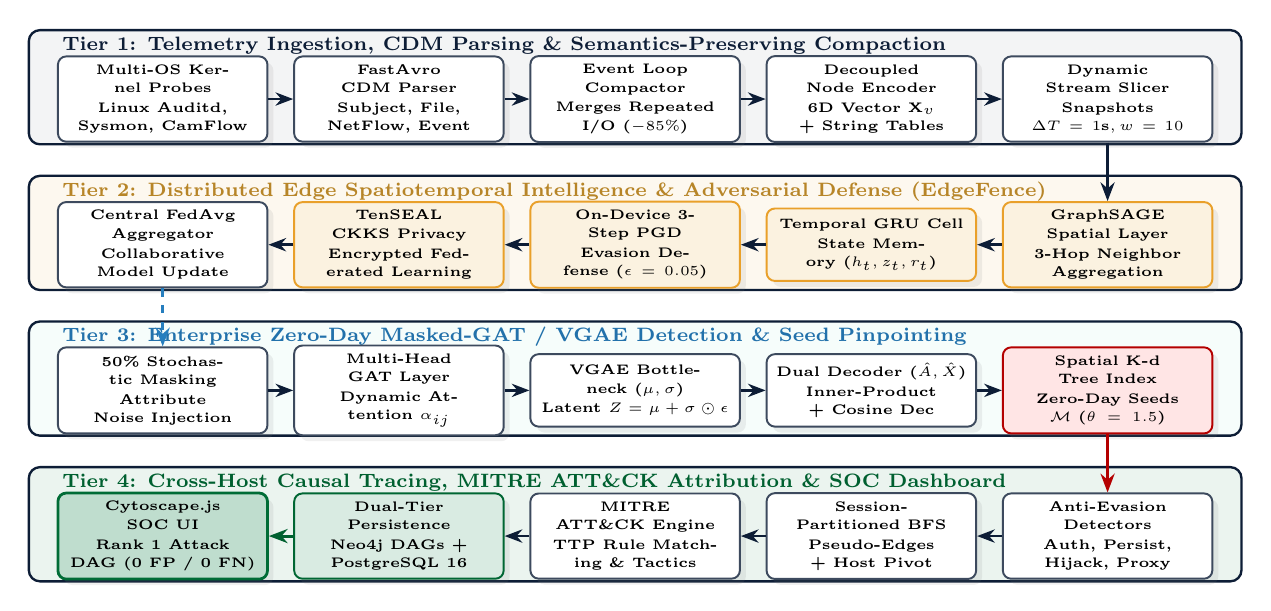
\begin{tikzpicture}[
  tier/.style={draw=prismNavy, rounded corners=4pt, line width=0.85pt, inner sep=4pt},
  comp/.style={draw=prismNavy!80, fill=white, rounded corners=3pt, line width=0.7pt,
               font=\fontsize{5.4}{6.6}\selectfont\bfseries, align=center, inner sep=3pt,
               text width=2.45cm, minimum height=0.92cm, drop shadow={opacity=0.12}},
  edgecomp/.style={draw=prismGold!85!orange, fill=prismGold!15, rounded corners=3pt, line width=0.7pt,
                   font=\fontsize{5.4}{6.6}\selectfont\bfseries, align=center, inner sep=3pt,
                   text width=2.45cm, minimum height=0.92cm, drop shadow={opacity=0.12}},
  soccomp/.style={draw=strengthGreen!85!black, fill=strengthGreen!15, rounded corners=3pt, line width=0.7pt,
                  font=\fontsize{5.4}{6.6}\selectfont\bfseries, align=center, inner sep=3pt,
                  text width=2.45cm, minimum height=0.92cm, drop shadow={opacity=0.12}},
  head/.style={font=\fontsize{6.6}{7.8}\selectfont\bfseries, align=left},
  arrow/.style={-{Stealth[scale=0.85]}, line width=1.0pt, color=prismNavy},
  darrow/.style={-{Stealth[scale=0.85]}, line width=1.0pt, dashed, color=prismBlue},
  greenarrow/.style={-{Stealth[scale=0.85]}, line width=1.1pt, color=strengthGreen!80!black}
]

% ======================================================================
% TIER 1: Telemetry Ingestion & Compaction (Top, Left to Right)
% ======================================================================
\node[tier, fill=prismNavy!5, minimum width=15.4cm, minimum height=1.45cm] (t1) at (0, 4.35) {};
\node[head, text=prismNavy, anchor=west] at (-7.4, 4.88) 
  {Tier 1: Telemetry Ingestion, CDM Parsing \& Semantics-Preserving Compaction};
\node[comp] (b1) at (-6.0, 4.20) {Multi-OS Kernel Probes\\[0.02cm]\tiny Linux Auditd, Sysmon, CamFlow};
\node[comp] (b2) at (-3.0, 4.20) {FastAvro CDM Parser\\[0.02cm]\tiny Subject, File, NetFlow, Event};
\node[comp] (b3) at (0.0, 4.20) {Event Loop Compactor\\[0.02cm]\tiny Merges Repeated I/O ($-85\%$)};
\node[comp] (b4) at (3.0, 4.20) {Decoupled Node Encoder\\[0.02cm]\tiny 6D Vector $\mathbf{X}_v$ + String Tables};
\node[comp] (b5) at (6.0, 4.20) {Dynamic Stream Slicer\\[0.02cm]\tiny Snapshots $\Delta T=1\text{s}, w=10$};

% ======================================================================
% TIER 2: Distributed Edge Intelligence (Right to Left)
% ======================================================================
\node[tier, fill=prismGold!8, minimum width=15.4cm, minimum height=1.45cm] (t2) at (0, 2.50) {};
\node[head, text=prismGold!80!black, anchor=west] at (-7.4, 3.03) 
  {Tier 2: Distributed Edge Spatiotemporal Intelligence \& Adversarial Defense (EdgeFence)};
\node[edgecomp] (b6) at (6.0, 2.35) {GraphSAGE Spatial Layer\\[0.02cm]\tiny 3-Hop Neighbor Aggregation};
\node[edgecomp] (b7) at (3.0, 2.35) {Temporal GRU Cell\\[0.02cm]\tiny State Memory ($h_t, z_t, r_t$)};
\node[edgecomp] (b8) at (0.0, 2.35) {On-Device 3-Step PGD\\[0.02cm]\tiny Evasion Defense ($\epsilon=0.05$)};
\node[edgecomp] (b9) at (-3.0, 2.35) {TenSEAL CKKS Privacy\\[0.02cm]\tiny Encrypted Federated Learning};
\node[comp] (b10) at (-6.0, 2.35) {Central FedAvg Aggregator\\[0.02cm]\tiny Collaborative Model Update};

% ======================================================================
% TIER 3: Enterprise Zero-Day Anomaly Detection (Left to Right)
% ======================================================================
\node[tier, fill=prismMint!30, minimum width=15.4cm, minimum height=1.45cm] (t3) at (0, 0.65) {};
\node[head, text=prismBlue!90!black, anchor=west] at (-7.4, 1.18) 
  {Tier 3: Enterprise Zero-Day Masked-GAT / VGAE Detection \& Seed Pinpointing};
\node[comp] (b11) at (-6.0, 0.50) {50\% Stochastic Masking\\[0.02cm]\tiny Attribute Noise Injection};
\node[comp] (b12) at (-3.0, 0.50) {Multi-Head GAT Layer\\[0.02cm]\tiny Dynamic Attention $\alpha_{ij}$};
\node[comp] (b13) at (0.0, 0.50) {VGAE Bottleneck ($\mu, \sigma$)\\[0.02cm]\tiny Latent $Z = \mu + \sigma \odot \epsilon$};
\node[comp] (b14) at (3.0, 0.50) {Dual Decoder ($\hat{A}, \hat{X}$)\\[0.02cm]\tiny Inner-Product + Cosine Dec};
\node[comp, draw=limitRed, fill=red!10] (b15) at (6.0, 0.50) {Spatial K-d Tree Index\\[0.02cm]\tiny Zero-Day Seeds $\mathcal{M}$ ($\theta=1.5$)};

% ======================================================================
% TIER 4: Cross-Host Causal Tracing & SOC Dashboard (Right to Left)
% ======================================================================
\node[tier, fill=strengthGreen!8, minimum width=15.4cm, minimum height=1.45cm] (t4) at (0, -1.20) {};
\node[head, text=strengthGreen!80!black, anchor=west] at (-7.4, -0.67) 
  {Tier 4: Cross-Host Causal Tracing, MITRE ATT\&CK Attribution \& SOC Dashboard};
\node[comp] (b16) at (6.0, -1.35) {Anti-Evasion Detectors\\[0.02cm]\tiny Auth, Persist, Hijack, Proxy};
\node[comp] (b17) at (3.0, -1.35) {Session-Partitioned BFS\\[0.02cm]\tiny Pseudo-Edges + Host Pivot};
\node[comp] (b18) at (0.0, -1.35) {MITRE ATT\&CK Engine\\[0.02cm]\tiny TTP Rule Matching \& Tactics};
\node[soccomp] (b19) at (-3.0, -1.35) {Dual-Tier Persistence\\[0.02cm]\tiny Neo4j DAGs + PostgreSQL 16};
\node[soccomp, fill=strengthGreen!25, draw=strengthGreen!90!black, line width=1.0pt] (b20) at (-6.0, -1.35) 
  {\textbf{Cytoscape.js SOC UI}\\[0.02cm]\tiny \textbf{Rank 1 Attack DAG (0 FP / 0 FN)}};

% ======================================================================
% HORIZONTAL INTRA-TIER CONNECTIONS
% ======================================================================
\draw[arrow] (b1) -- (b2);
\draw[arrow] (b2) -- (b3);
\draw[arrow] (b3) -- (b4);
\draw[arrow] (b4) -- (b5);

\draw[arrow] (b6) -- (b7);
\draw[arrow] (b7) -- (b8);
\draw[arrow] (b8) -- (b9);
\draw[arrow] (b9) -- (b10);

\draw[arrow] (b11) -- (b12);
\draw[arrow] (b12) -- (b13);
\draw[arrow] (b13) -- (b14);
\draw[arrow] (b14) -- (b15);

\draw[arrow] (b16) -- (b17);
\draw[arrow] (b17) -- (b18);
\draw[arrow] (b18) -- (b19);
\draw[greenarrow] (b19) -- (b20);

% ======================================================================
% VERTICAL INTER-TIER CONNECTORS (PURE VERTICAL - ZERO CROSSING)
% ======================================================================
% Tier 1 to Tier 2 (Right Side)
\draw[arrow, line width=1.1pt] (b5) -- (b6);

% Tier 2 to Tier 3 (Left Side)
\draw[darrow, line width=1.1pt] (b10) -- (b11);

% Tier 3 to Tier 4 (Right Side)
\draw[arrow, line width=1.1pt, color=limitRed] (b15) -- (b16);

\end{tikzpicture}}
\end{frame}

%% ======================================================================
%%  14. PROJECT DEVELOPMENT AND TESTING FLOWCHART
%% ======================================================================
\section{Project Development \& Testing Flowchart}

\begin{frame}{14. Project Development and Testing Flowchart}
\vspace{-0.15em}
\centering
\resizebox{0.98\textwidth}{!}{%
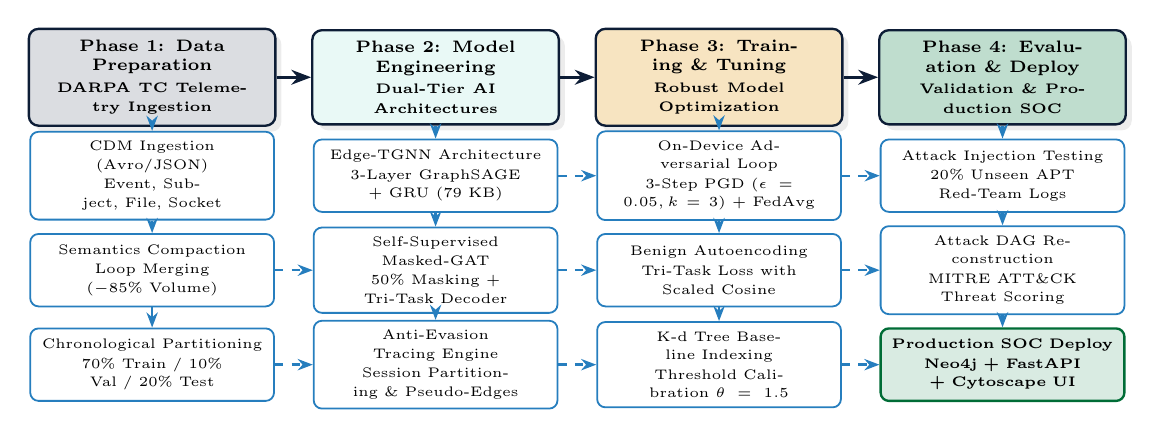
\begin{tikzpicture}[
  stage/.style={draw=prismNavy, rounded corners=3.5pt, line width=0.85pt,
                font=\fontsize{6.0}{7.0}\selectfont\bfseries, align=center, inner sep=4pt,
                text width=2.85cm, minimum height=0.88cm, drop shadow={opacity=0.15}},
  stepbox/.style={draw=prismBlue, fill=white, rounded corners=3pt, line width=0.65pt,
                  font=\fontsize{5.4}{6.6}\selectfont, align=center, inner sep=3.5pt,
                  text width=2.85cm, minimum height=0.92cm},
  flowarrow/.style={-{Stealth[scale=0.90]}, line width=1.1pt, color=prismNavy},
  subarrow/.style={-{Stealth[scale=0.80]}, line width=0.85pt, color=prismBlue}
]

% Phase Headers (Row 0)
\node[stage, fill=prismNavy!15] (p1) at (0, 0) {Phase 1: Data Preparation\\[0.03cm]\tiny DARPA TC Telemetry Ingestion};
\node[stage, fill=prismMint!70] (p2) at (3.6, 0) {Phase 2: Model Engineering\\[0.03cm]\tiny Dual-Tier AI Architectures};
\node[stage, fill=prismGold!30] (p3) at (7.2, 0) {Phase 3: Training \& Tuning\\[0.03cm]\tiny Robust Model Optimization};
\node[stage, fill=strengthGreen!25] (p4) at (10.8, 0) {Phase 4: Evaluation \& Deploy\\[0.03cm]\tiny Validation \& Production SOC};

% Row 1: Core Architectures & Training
\node[stepbox] (s1) at (0, -1.25) {CDM Ingestion (Avro/JSON)\\[0.02cm]\tiny Event, Subject, File, Socket};
\node[stepbox] (s4) at (3.6, -1.25) {Edge-TGNN Architecture\\[0.02cm]\tiny 3-Layer GraphSAGE + GRU (79~KB)};
\node[stepbox] (s7) at (7.2, -1.25) {On-Device Adversarial Loop\\[0.02cm]\tiny 3-Step PGD ($\epsilon=0.05, k=3$) + FedAvg};
\node[stepbox] (s10) at (10.8, -1.25) {Attack Injection Testing\\[0.02cm]\tiny 20\% Unseen APT Red-Team Logs};

% Row 2: Compaction, Masked-GAT & Evaluation
\node[stepbox] (s2) at (0, -2.45) {Semantics Compaction\\[0.02cm]\tiny Loop Merging ($-85\%$ Volume)};
\node[stepbox] (s5) at (3.6, -2.45) {Self-Supervised Masked-GAT\\[0.02cm]\tiny 50\% Masking + Tri-Task Decoder};
\node[stepbox] (s8) at (7.2, -2.45) {Benign Autoencoding\\[0.02cm]\tiny Tri-Task Loss with Scaled Cosine};
\node[stepbox] (s11) at (10.8, -2.45) {Attack DAG Reconstruction\\[0.02cm]\tiny MITRE ATT\&CK Threat Scoring};

% Row 3: Partitions, Anti-Evasion & Production Deploy
\node[stepbox] (s3) at (0, -3.65) {Chronological Partitioning\\[0.02cm]\tiny 70\% Train / 10\% Val / 20\% Test};
\node[stepbox] (s6) at (3.6, -3.65) {Anti-Evasion Tracing Engine\\[0.02cm]\tiny Session Partitioning \& Pseudo-Edges};
\node[stepbox] (s9) at (7.2, -3.65) {K-d Tree Baseline Indexing\\[0.02cm]\tiny Threshold Calibration $\theta=1.5$};
\node[stepbox, fill=strengthGreen!15, draw=strengthGreen!90!black, line width=0.85pt] (s12) at (10.8, -3.65) 
  {\textbf{Production SOC Deploy}\\[0.02cm]\tiny \textbf{Neo4j + FastAPI + Cytoscape UI}};

% Phase Header Connectors (Horizontal)
\draw[flowarrow] (p1) -- (p2);
\draw[flowarrow] (p2) -- (p3);
\draw[flowarrow] (p3) -- (p4);

% Vertical Intra-Phase Connectors
\draw[subarrow] (p1) -- (s1); \draw[subarrow] (s1) -- (s2); \draw[subarrow] (s2) -- (s3);
\draw[subarrow] (p2) -- (s4); \draw[subarrow] (s4) -- (s5); \draw[subarrow] (s5) -- (s6);
\draw[subarrow] (p3) -- (s7); \draw[subarrow] (s7) -- (s8); \draw[subarrow] (s8) -- (s9);
\draw[subarrow] (p4) -- (s10); \draw[subarrow] (s10) -- (s11); \draw[subarrow] (s11) -- (s12);

% Horizontal Inter-Phase Transition Connectors
\draw[subarrow, dashed] (s4) -- (s7);
\draw[subarrow, dashed] (s7) -- (s10);

\draw[subarrow, dashed] (s2) -- (s5);
\draw[subarrow, dashed] (s5) -- (s8);
\draw[subarrow, dashed] (s8) -- (s11);

\draw[subarrow, dashed] (s3) -- (s6);
\draw[subarrow, dashed] (s6) -- (s9);
\draw[subarrow, dashed] (s9) -- (s12);

\end{tikzpicture}}
\end{frame}

%% ======================================================================
%%  15. DATABASE SCHEMA
%% ======================================================================
\section{Database Schema}

\begin{frame}{15. Database Schema: Neo4j Graph Database Property Schema}
\vspace{0.3em}
\begin{beamercolorbox}[rounded=true,shadow=false,sep=0.45em,wd=\textwidth]{block title}
\textbf{\scriptsize 1. Neo4j Graph Database Property Schema (Whole-System Provenance)}
\end{beamercolorbox}
\vspace{0.3em}
{\fontsize{7.8pt}{11.2pt}\selectfont
\textbf{Node Labels \& Key Properties:}
\begin{itemize}\itemsep0.30em
  \item \textbf{\texttt{:Process}}: \texttt{\{uuid, pid, name, path, cmdline, uid, session\_id, host\}}
  \item \textbf{\texttt{:File}}: \texttt{\{uuid, path, name, file\_type, size\_bytes, permissions, hash\}}
  \item \textbf{\texttt{:Socket}}: \texttt{\{uuid, src\_ip, src\_port, dst\_ip, dst\_port, protocol\}}
  \item \textbf{\texttt{:Controller}}: \texttt{\{uuid, model, ip, protocol, firmware, trip\_curve\}}
\end{itemize}
\vspace{0.3em}
\textbf{Directed Relationship Types \& Causal Edges:}
\begin{itemize}\itemsep0.30em
  \item \textbf{\texttt{[:FORK | :EXEC]}}: \texttt{(Process) $\rightarrow$ (Process/File) \{timestamp\}}
  \item \textbf{\texttt{[:READ | :WRITE]}}: \texttt{(Process) $\rightarrow$ (File) \{timestamp, count\}}
  \item \textbf{\texttt{[:CONNECT]}}: \texttt{(Process) $\rightarrow$ (Socket) \{timestamp, state\}}
  \item \textbf{\texttt{[:PERSISTENCE\_PSEUDO\_EDGE]}}: \texttt{(SetupSession) $\rightarrow$ (ExecSession)}
  \item \textbf{\texttt{[:PORTFWD\_CROSS\_MACHINE]}}: \texttt{(ProxySrc) $\rightarrow$ (TargetDst)}
\end{itemize}
}
\end{frame}

\begin{frame}{15. Database Schema: Relational Metadata Store (PostgreSQL)}
\vspace{0.3em}
\begin{beamercolorbox}[rounded=true,shadow=false,sep=0.45em,wd=\textwidth]{block title}
\textbf{\scriptsize 2. Relational Metadata Store (PostgreSQL 16 Tables)}
\end{beamercolorbox}
\vspace{0.3em}
{\fontsize{7.8pt}{11.5pt}\selectfont
\begin{itemize}\itemsep0.45em
  \item \textbf{\texttt{hosts} (Endpoint Inventory):}\\
  Tracks connected infrastructure with schema:
  \begin{itemize}\itemsep0.15em
    \item \texttt{host\_id} (PK), \texttt{hostname}, \texttt{os\_platform}, \texttt{domain\_name}, \texttt{ip\_addr}, \texttt{is\_dc}, \texttt{last\_seen}
  \end{itemize}
  \item \textbf{\texttt{anomalies} (AI-Flagged Seed Events):}\\
  Persists detected anomaly seeds from Edge-TGNN and Masked-GAT:
  \begin{itemize}\itemsep0.15em
    \item \texttt{anomaly\_id} (PK), \texttt{host\_id} (FK), \texttt{session\_id}, \texttt{score}, \texttt{detector\_source}, \texttt{timestamp}
  \end{itemize}
  \item \textbf{\texttt{attack\_graphs} (Reconstructed Scenarios):}\\
  Stores causal DAGs with complete MITRE ATT\&CK mapping:
  \begin{itemize}\itemsep0.15em
    \item \texttt{graph\_id} (PK), \texttt{seed\_uuid}, \texttt{threat\_score}, \texttt{tactics\_list}, \texttt{node\_count}, \texttt{edge\_count}, \texttt{graph\_json}
  \end{itemize}
  \item \textbf{\texttt{federated\_updates} (Collaborative Training Logs):}\\
  Records parameter norms and loss deltas across federated aggregation rounds:
  \begin{itemize}\itemsep0.15em
    \item \texttt{round\_id} (PK), \texttt{client\_id}, \texttt{loss\_clean}, \texttt{loss\_adv}, \texttt{param\_norm}, \texttt{timestamp}
  \end{itemize}
\end{itemize}
}
\end{frame}

%% ======================================================================
%%  16. ALGORITHMS AND PSEUDOCODE
%% ======================================================================
\section{Algorithms and Pseudocode}

\begin{frame}{16. Master Algorithm: Unified End-to-End Threat Detection Pipeline}
\vspace{-0.30em}
\begin{beamercolorbox}[rounded=true,shadow=false,sep=0.25em,wd=\textwidth]{block title}
\textbf{\scriptsize Master Pipeline: Orchestrating All 5 Project Working Phases}
\end{beamercolorbox}
\vspace{0.08em}
{\fontsize{6.0pt}{7.5pt}\selectfont
\textbf{Intuition:} Synchronizes data ingestion, event loop compaction, real-time edge screening, central zero-day pinpointing, and cross-machine causal tracing into a unified defense pipeline.
}
\vspace{0.10em}
\centering
\begin{beamercolorbox}[rounded=true,shadow=false,sep=0.20em,wd=0.98\textwidth]{codeBg}
{\fontsize{4.8pt}{5.8pt}\selectfont\ttfamily
\textbf{Master Algorithm: Complete Threat Detection \& Scenario Reconstruction}\\
\textbf{Input:} Raw Audit Telemetry Stream $\mathcal{S}_{\text{audit}}$, Auth Logs $\mathcal{A}$, Baseline Profile $\mathcal{D}_{\text{norm}}$, TTP Rules $\mathcal{R}$.\\
\textbf{Output:} Ranked list of prioritized multi-host Attack Scenario DAGs $\mathcal{L}_{\langle AG, TS \rangle}$.\\[0.03cm]
\rule{\linewidth}{0.3pt}\\[0.03cm]
1: \textit{// Phase 1: Ingestion \& Semantics-Preserving Compaction}\\
2: Ingest CDM records (Subject, File, NetFlow, Event); Collapse repetitive loops: $w(e) \leftarrow w(e)+1$ ($-85\%$ volume).\\
3: Slice stream into rolling snapshot graph windows $G_{i,t,w} = \{G_{t-9}, \dots, G_t\}$ with $\Delta T=1.0\text{ s}, w=10$.\\
4: \textit{// Phase 2: First-Line Edge Anomaly Screening (Algorithm 1: EdgeFence)}\\
5: Forward $G_{i,t,w}$ through on-device Edge-TGNN: $s_{i,t} \leftarrow \sigma(W_{\text{out}} \text{GRU}(h_{G_t}) + b)$ in $<4$~ms.\\
6: \textbf{if} $s_{i,t} > \tau_{\text{edge}}$ \textbf{then} Dispatch high-priority alert; Transmit compacted subgraph $G_{\text{anom}}$ to SOC cluster.\\
7: \textit{// Phase 3: Self-Supervised Zero-Day Seed Detection (Algorithm 2: MGDA)}\\
8: Pass $G_{\text{anom}}$ into Masked-GAT autoencoder; Reconstruct 50\% masked node attributes: $\hat{X} \leftarrow f_D(f_E(\tilde{X}, E))$.\\
9: Query K-d tree normal baseline memory ($k=10$); Compute normalized outlier score: $\text{Score}(v) = \frac{\bar{D}_{\text{test}}(h_v)}{\bar{D}_{\text{train}}}$.\\
10:Extract set of malicious seed process entities: $\mathcal{M} \leftarrow \{v \mid \text{Score}(v) \ge \theta \text{ and type}(v) == \text{Process}\}$.\\
11:\textit{// Phase 4: Cross-Machine Tracing \& Pseudo-Edge Resolution (Algorithm 3: Commander)}\\
12:Run 4 preliminary detectors: Authentication anomaly, persistence, session hijack, and port forwarding proxy.\\
13:\textbf{for} each seed $v \in \mathcal{M}$ \textbf{do}: Identify LogonSessionID; Insert pseudo-edges; Perform bidirectional BFS.\\
14:\textbf{if} gateway / jump-server session is traversed \textbf{then} Trace across IT domain into OT industrial controller logs.\\
15:\textit{// Phase 5: MITRE ATT\&CK Annotation and Threat Score Calculation}\\
16:Match graph paths against TTP rules $\mathcal{R}$; Annotate tactics; Compute $TS_{\text{total}} = \sum TS_{\text{edge}} \cdot (1+DA) \cdot Crit$.\\
17:\textbf{return} Ranked list $\mathcal{L}_{\langle AG, TS \rangle}$ sorted descending by $TS_{\text{total}}$ (Surfacing true attack at \textbf{Rank 1}).
}
\end{beamercolorbox}
\end{frame}

\begin{frame}{16. Algorithm 1: On-Device Federated Adversarial TGNN Training}
\vspace{-0.30em}
\begin{beamercolorbox}[rounded=true,shadow=false,sep=0.25em,wd=\textwidth]{block title}
\textbf{\scriptsize Phase I Algorithm: On-Device Edge-TGNN Training with Adversarial Hardening (EdgeFence)}
\end{beamercolorbox}
\vspace{0.08em}
{\fontsize{6.0pt}{7.5pt}\selectfont
\textbf{Intuition:} Protects edge models against attacker evasion tricks (dummy syscall additions) via 3-step PGD, while TenSEAL CKKS encrypted FedAvg preserves employee data privacy.
}
\vspace{0.10em}
\centering
\begin{beamercolorbox}[rounded=true,shadow=false,sep=0.20em,wd=0.98\textwidth]{codeBg}
{\fontsize{4.8pt}{5.8pt}\selectfont\ttfamily
\textbf{Algorithm 1: Federated Adversarial TGNN Training}\\
\textbf{Input:} Clients $\mathcal{S}=\{1,\dots,N\}$, Local datasets $\mathcal{D}_i$, Rounds $R=100$, Local Epochs $E=1$, Learning rate $\eta=0.001$, PGD steps $K_{\text{att}}=3$, Bound $\epsilon=0.05$, Edge budget $k_{\text{mod}}=3$, Adv weight $\lambda=0.8$.\\
\textbf{Output:} Adversarially Hardened Global Model $\theta^{(R)}$ ($<80$~KB).\\[0.03cm]
\rule{\linewidth}{0.3pt}\\[0.03cm]
1: Central Server initializes global model $\theta^{(0)}$ ($\sim 79.63\text{ KB}$).\\
2: \textbf{for} each federated round $r = 1, \dots, R$ \textbf{do}:\\
3: \quad Server selects client subset $\mathcal{S}^{(r)} \subseteq \{1,\dots,N\}$ of size $S_{\text{rate}} \cdot N$ ($S_{\text{rate}}=0.1$).\\
4: \quad Server broadcasts current global parameters $\theta^{(r)}$ to selected clients.\\
5: \quad \textbf{for} each client $i \in \mathcal{S}^{(r)}$ \textbf{in parallel do}:\\
6: \qquad Initialize local parameters $\theta_i \leftarrow \theta^{(r)}$.\\
7: \qquad \textbf{for} each local epoch $e = 1$ to $E$ \textbf{do}:\\
8: \qquad \quad \textbf{for} each mini-batch $(G_T, y) \in \mathcal{D}_i$ \textbf{do}:\\
9: \qquad \qquad \textit{// 1. On-Device PGD Adversarial Perturbation Generation:}\\
10:\qquad \qquad Initialize $\delta \leftarrow 0$; \textbf{for} step $= 1$ to $K_{\text{att}}$ \textbf{do}: $\delta \leftarrow \text{clip}\left(\delta + \alpha \cdot \text{sgn}(\nabla_\delta \ell(f_{\theta_i}(G_T + \delta), y)), -\epsilon, \epsilon\right)$; Project discrete edges $\le k_{\text{mod}}$.\\
11:\qquad \qquad Generate adversarial graph sequence: $G_T' \leftarrow G_T + \delta^*$.\\
12:\qquad \qquad \textit{// 2. Composite Loss Minimization:}\\
13:\qquad \qquad $\mathcal{L}_i^{\text{adv}} = \text{BCE}(f_{\theta_i}(G_T), y) + \lambda \cdot \text{BCE}(f_{\theta_i}(G_T'), y)$.\\
14:\qquad \qquad Update weights: $\theta_i \leftarrow \theta_i - \eta \nabla_{\theta_i} \mathcal{L}_i^{\text{adv}}$ using Adam optimizer.\\
15:\qquad Compute parameter delta: $\Delta \theta_i^{(r)} \leftarrow \theta_i - \theta^{(r)}$; Upload $\Delta \theta_i^{(r)}$ via TenSEAL CKKS to Server.\\
16:\quad Server performs FedAvg aggregation: $\theta^{(r+1)} \leftarrow \theta^{(r)} + \sum_{i \in \mathcal{S}^{(r)}} \frac{|\mathcal{D}_i|}{\sum |\mathcal{D}_j|} \Delta \theta_i^{(r)}$.\\
17:\textbf{return} Final Hardened Global Model $\theta^{(R)}$.
}
\end{beamercolorbox}
\end{frame}

\begin{frame}{16. Algorithm 2: Self-Supervised Masked-GAT Autoencoder \& Outlier Detection}
\vspace{-0.30em}
\begin{beamercolorbox}[rounded=true,shadow=false,sep=0.25em,wd=\textwidth]{block title}
\textbf{\scriptsize Phase II Algorithm: Self-Supervised Masked-GAT \& K-d Tree Outlier Detection (MGDA)}
\end{beamercolorbox}
\vspace{0.08em}
{\fontsize{6.0pt}{7.5pt}\selectfont
\textbf{Intuition:} Learns normal system baseline behavior from 100\% benign execution logs; isolates unknown zero-day attack seeds when reconstruction distance exceeds the normal K-d tree neighborhood.
}
\vspace{0.10em}
\centering
\begin{beamercolorbox}[rounded=true,shadow=false,sep=0.20em,wd=0.98\textwidth]{codeBg}
{\fontsize{4.8pt}{5.8pt}\selectfont\ttfamily
\textbf{Algorithm 2: Self-Supervised Training and K-d Tree Outlier Detection}\\
\textbf{Input:} Compressed Provenance Graph $G = (V, E, X)$, Mask Ratio $\rho=0.5$, Re-mask Views $K=3$, Scaling Exponent $\gamma=2.0$, Neighbors $k=10$, Outlier Threshold $\theta=1.5$.\\
\textbf{Output:} Set of Malicious Seed Process Entities $\mathcal{M}$.\\[0.03cm]
\rule{\linewidth}{0.3pt}\\[0.03cm]
1: \textit{// Phase A: Self-Supervised Training on Benign Baseline Graphs:}\\
2: Initialize GAT Encoder $f_E$, Feature Decoder $f_D$, Latent Projector $g$, Edge Predictor MLP, Target Generator $f_T$.\\
3: \textbf{for} epoch $= 1$ to $E_{\text{train}}$ \textbf{do}:\\
4: \quad Randomly sample 50\% nodes $\tilde{V} \subset V$; Replace features: $\tilde{X}_i \leftarrow [MASK]$ for $v_i \in \tilde{V}$.\\
5: \quad Forward corrupted graph through GAT: $H \leftarrow f_E(\tilde{X}, E) = h^{(1)} \parallel h^{(2)} \parallel h^{(3)}$.\\
6: \quad \textit{// Task 1: Multi-view random re-mask decoding:}\\
7: \quad Compute $\mathcal{L}_{\text{input}} = \frac{1}{K}\sum_{k=1}^K \sum_{v_i \in \tilde{V}} (1 - \cos(x_i, f_D(\bar{H}^{(k)})))^\gamma$.\\
8: \quad \textit{// Task 2: Latent target representation prediction:}\\
9: \quad Compute target $Z \leftarrow f_T(X, E)$; Compute $\mathcal{L}_{\text{latent}} = \sum_{v_i \in \tilde{V}} (1 - \cos(z_i, g(H_i)))^\gamma$.\\
10:\quad \textit{// Task 3: Structure Edge Prediction:}\\
11:\quad Predict positive edges $E^+$ and negative pairs $E^-$: $\mathcal{L}_{\text{struct}} = \text{BCE}(\text{MLP}([H_u \parallel H_v]), Y_{\text{edge}})$.\\
12:\quad Optimize total loss: $\mathcal{L}_{\text{total}} = \mathcal{L}_{\text{input}} + \mathcal{L}_{\text{latent}} + 0.5 \mathcal{L}_{\text{struct}}$ via Adam.\\
13:\textit{// Phase B: K-d Tree Indexing and Anomaly Scoring:}\\
14:Extract all benign node representations $H_{\text{train}}$; Index into K-d Tree $\mathcal{T}$.\\
15:\textbf{for} each entity embedding $h_v \in H_{\text{test}}$ \textbf{do}:\\
16:\quad Query $\mathcal{T}$ for $k=10$ nearest neighbors; Compute normalized outlier score: $\text{Score}(v) = \frac{\bar{D}_{\text{test}}(h_v)}{\bar{D}_{\text{train\_neighbors}}}$.\\
17:\quad \textbf{if} $\text{Score}(v) \ge \theta$ \textbf{and} $\text{type}(v) == \text{Process}$ \textbf{then} $\mathcal{M} \leftarrow \mathcal{M} \cup \{v\}$.\\
18:\textbf{return} Malicious Seed Nodes $\mathcal{M}$.
}
\end{beamercolorbox}
\end{frame}

\begin{frame}{16. Algorithm 3: Cross-Machine Attack Graph Tracing \& Scenario Reconstruction}
\vspace{-0.30em}
\begin{beamercolorbox}[rounded=true,shadow=false,sep=0.25em,wd=\textwidth]{block title}
\textbf{\scriptsize Phase III Algorithm: Cross-Machine Tracing \& MITRE Attribution (Commander)}
\end{beamercolorbox}
\vspace{0.08em}
{\fontsize{6.0pt}{7.5pt}\selectfont
\textbf{Intuition:} Bounded bidirectional BFS tracks multi-host attacker movement without graph explosion; pseudo-edges connect persistence setups, token duplication, and proxy tunnels.
}
\vspace{0.10em}
\centering
\begin{beamercolorbox}[rounded=true,shadow=false,sep=0.20em,wd=0.98\textwidth]{codeBg}
{\fontsize{4.8pt}{5.8pt}\selectfont\ttfamily
\textbf{Algorithm 3: Robust Whole-Network Tracing and ATT\&CK Reconstruction}\\
\textbf{Input:} Audit events $\mathcal{E}$, Authentication logs $\mathcal{A}$, Malicious Seeds $\mathcal{M}$, TTP Rules $\mathcal{R}_{\text{Host}}, \mathcal{R}_{\text{Net}}$.\\
\textbf{Output:} Ranked list of Attack Graphs and Threat Scores $\mathcal{L}_{\langle AG, TS \rangle}$.\\[0.03cm]
\rule{\linewidth}{0.3pt}\\[0.03cm]
1: Run 4 Preliminary Detectors in parallel:\\
2: \quad $\mathcal{L}_{\text{auth}} \leftarrow \text{DetectAuthenticationAnomaly}(\mathcal{A})$; \quad $\mathcal{L}_{\text{pers}} \leftarrow \text{DetectPersistence}(\mathcal{E})$;\\
3: \quad $\mathcal{L}_{\text{hijack}} \leftarrow \text{DetectSessionHijacking}(\mathcal{E}, \mathcal{A})$; \quad $\mathcal{L}_{\text{portfwd}} \leftarrow \text{DetectPortForwarding}(\mathcal{E}, \mathcal{A})$.\\
4: \textbf{for} each anomaly in $\mathcal{L}_{\text{auth}} \cup \mathcal{M}$ \textbf{do}:\\
5: \quad Initialize Attack Graph $AG \leftarrow \text{CreateHighLevelGraph}(\text{seed})$; Identify $AccessType \leftarrow \text{CheckRemoteAccess}(\mathcal{E})$.\\
6: \quad $SessionID \leftarrow \text{ReassignSessionID}(AccessType)$; Link child user session to parent service session.\\
7: \quad \textit{// Intra-Machine Backward \& Forward Traversal with Pseudo-Edges:}\\
8: \quad $(E_\alpha, G_\alpha) \leftarrow \text{TraverseBackward}(SessionID, \mathcal{E}, \mathcal{L}_{\text{pers}}, \mathcal{L}_{\text{hijack}}, \mathcal{L}_{\text{portfwd}})$.\\
9: \quad $(E_\kappa, G_\kappa) \leftarrow \text{TraverseForward}(SessionID, \mathcal{E}, \mathcal{L}_{\text{pers}}, \mathcal{L}_{\text{hijack}}, \mathcal{L}_{\text{portfwd}})$.\\
10:\quad $AG \leftarrow AG \cup G_\alpha \cup G_\kappa$.\\
11:\quad \textit{// Cross-Machine \& Cross-Host Network Tracing:}\\
12:\quad \textbf{if} cross-host socket / SSH connection is involved \textbf{then} Trace across enterprise network hosts via network provenance edges.\\
13:\quad \textit{// Multi-Stage Lateral Movement Resolution:}\\
14:\quad \textbf{if} remote logon session detected \textbf{then} Correlate remote host provenance DAGs; Map enterprise MITRE ATT\&CK TTPs.\\
15:\quad \textit{// ATT\&CK Annotation and Threat Score Calculation:}\\
16:\quad Annotate edges with MITRE TTPs; Compute $TS_{\text{edge}} = \sum w_i [Freq(teq_i) + Var(tac_i)]$.\\
17:\quad Compute $TS_{\text{total}} = \sum TS_{\text{edge}} \cdot (1 + DA) \cdot Criticality$.\\
18:\quad $\mathcal{L}_{\langle AG, TS \rangle} \leftarrow \mathcal{L}_{\langle AG, TS \rangle} \cup (AG, TS_{\text{total}})$.\\
19:\textbf{return} $\mathcal{L}_{\langle AG, TS \rangle}$ sorted descending by $TS_{\text{total}}$.
}
\end{beamercolorbox}
\end{frame}


%% ======================================================================
%%  17. IMPLEMENTATION & TECHNOLOGY STACK
%% ======================================================================
\section{Implementation \& Technology Stack}

\begin{frame}{17. Implementation: Core System Modules \& Architecture}
\vspace{0.3em}
\begin{beamercolorbox}[rounded=true,shadow=false,sep=0.45em,wd=\textwidth]{block title}
\textbf{\scriptsize 1. Core Engineering Modules \& Functional Pipeline}
\end{beamercolorbox}
\vspace{0.3em}
{\fontsize{7.8pt}{11.5pt}\selectfont
\begin{itemize}\itemsep0.45em
  \item \textbf{Kernel Ingestion \& Parsing Engine:}\\
  Low-overhead audit probe hooks (Linux \texttt{auditd}, CamFlow LSM hooks, Windows Sysmon v14). Ingests raw audit logs and converts to CDM JSON/Avro records in real time.
  \item \textbf{Semantics-Preserving Event Compactor:}\\
  High-throughput Rust/Python microservice evaluating execution state equivalence and collapsing repetitive I/O loops (reduces raw volume $>85\%$).
  \item \textbf{Dual-Tier AI Detection Server:}\\
  PyTorch Geometric microservice running lightweight Edge-TGNN ($79.63$~KB) on edge gateways and centralized self-supervised Masked-GAT on GPU cluster.
  \item \textbf{Whole-Network Causal Tracing Engine:}\\
  Logon-session partitioned DFS/BFS crawler inserting pseudo-edges to bridge persistence, token hijacking, and reverse proxy tunnels across hosts.
\end{itemize}
}
\end{frame}

\begin{frame}{17. Implementation: Technology Stack \& Frameworks}
\vspace{0.2em}
\begin{beamercolorbox}[rounded=true,shadow=false,sep=0.40em,wd=\textwidth]{block title}
\textbf{\scriptsize 2. Technology Stack, Libraries \& Frameworks}
\end{beamercolorbox}
\vspace{0.2em}
{\fontsize{7.6pt}{11.0pt}\selectfont
\begin{itemize}\itemsep0.32em
  \item \textbf{Deep Learning \& Graph Frameworks:}\\
  Python 3.10+, PyTorch v2.2.0, PyTorch Geometric (PyG v2.5.0), DGL v1.1, SciPy v1.12 (K-d Tree spatial index), NumPy, and Scikit-Learn.
  \item \textbf{Privacy-Preserving Federated Cryptography:}\\
  \textbf{TenSEAL CKKS Homomorphic Encryption} for encrypted parameter aggregation in Federated Learning without gradient or data leakage.
  \item \textbf{Dual-Tier Database \& Graph Storage Engines:}\\
  \textbf{Neo4j Enterprise 5.x} with Cypher query interface and APOC graph algorithms for high-speed DAG indexing; \textbf{PostgreSQL 16} for metadata and relational state.
  \item \textbf{Telemetry Sensors \& Serialization:}\\
  FastAvro v1.9 for binary CDM decoding, Linux Auditd, CamFlow v0.5 LSM hooks, and Windows Sysmon v14 with Event Forwarding.
  \item \textbf{Forensic Dashboard \& API:}\\
  \textbf{FastAPI} async REST API backend; \textbf{Cytoscape.js} interactive graph canvas for SOC triage and multi-stage DAG exploration.
\end{itemize}
}
\end{frame}

%% ======================================================================
%%  WORK PLAN & GANTT CHART
%% ======================================================================
\section{Work Plan \& Gantt Chart}

\begin{frame}{18. Project Work Plan \& Gantt Chart Roadmap}
\vspace{-0.15em}
\centering
\resizebox{\textwidth}{!}{%
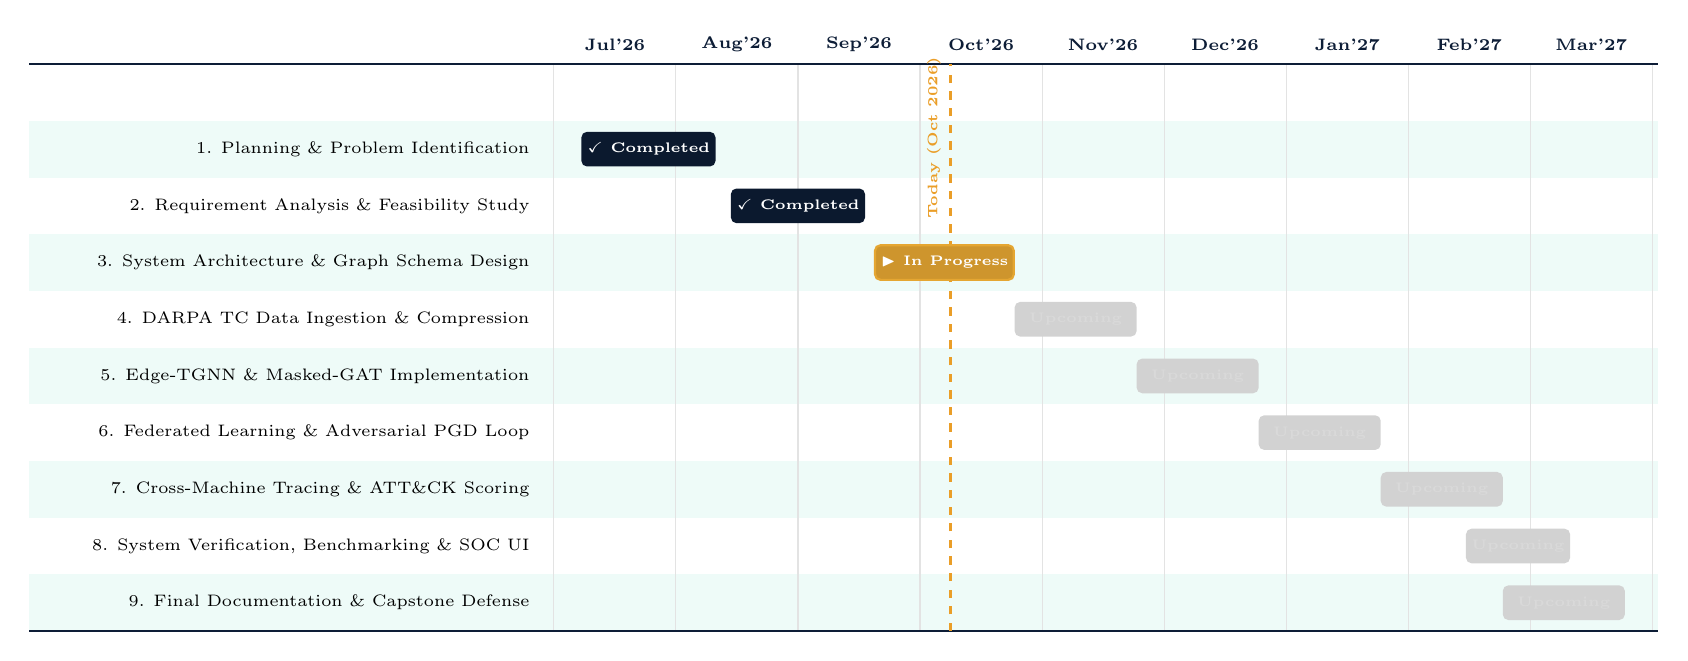
\begin{tikzpicture}[
  x=1.55cm, y=0.72cm,
  done/.style  ={rounded corners=2pt, minimum height=0.44cm, inner sep=2pt,
                 font=\fontsize{5.2}{6}\selectfont\bfseries\color{white},
                 fill=prismNavy!85!black},
  now/.style   ={rounded corners=2pt, minimum height=0.44cm, inner sep=2pt,
                 font=\fontsize{5.2}{6}\selectfont\bfseries\color{white},
                 fill=prismGold!90!black, draw=prismGold, line width=0.8pt},
  future/.style={rounded corners=2pt, minimum height=0.44cm, inner sep=2pt,
                 font=\fontsize{5.2}{6}\selectfont\bfseries\color{white!70!gray},
                 fill=gray!35},
  hdr/.style={font=\fontsize{6.5}{7.5}\selectfont\bfseries, text=prismNavy},
  lbl/.style={font=\fontsize{6.5}{7.5}\selectfont, text=black, anchor=east},
  gl/.style={draw=gray!22, line width=0.4pt},
  stripe/.style={fill=prismMint!55}
]
\foreach \r in {1,3,5,7,9} { \fill[stripe] (-4.3,\r-0.5) rectangle (9.05,\r+0.5); }
\foreach \col/\mo in {0/{Jul'26},1/{Aug'26},2/{Sep'26},3/{Oct'26},4/{Nov'26},5/{Dec'26},6/{Jan'27},7/{Feb'27},8/{Mar'27}} {
  \draw[gl] (\col, 0.5) -- (\col, 10.5);
  \node[hdr] at (\col+0.5, 10.85) {\mo};
}
\draw[gl] (9.0, 0.5) -- (9.0, 10.5);
\draw[prismNavy, line width=1.0pt] (-4.3, 10.5) -- (9.05, 10.5);
\draw[prismNavy, line width=0.5pt] (-4.3, 0.5)  -- (9.05, 0.5);
\draw[prismGold!80!orange, line width=1.4pt, dashed] (3.25, 0.5) -- (3.25, 10.5);
\node[font=\fontsize{5.2}{6}\selectfont\bfseries, text=prismGold!80!orange, rotate=90, anchor=south] at (3.25, 9.2) {Today (Oct 2026)};
\node[lbl] at (-0.12, 9) {1. Planning \& Problem Identification};
\node[done, minimum width=1.55cm] at (0.775, 9) {\checkmark\ Completed};
\node[lbl] at (-0.12, 8) {2. Requirement Analysis \& Feasibility Study};
\node[done, minimum width=1.55cm] at (2.00, 8) {\checkmark\ Completed};
\node[lbl] at (-0.12, 7) {3. System Architecture \& Graph Schema Design};
\node[now, minimum width=1.55cm] at (3.20, 7) {$\blacktriangleright$ In Progress};
\node[lbl] at (-0.12, 6) {4. DARPA TC Data Ingestion \& Compression};
\node[future, minimum width=1.55cm] at (4.275, 6) {Upcoming};
\node[lbl] at (-0.12, 5) {5. Edge-TGNN \& Masked-GAT Implementation};
\node[future, minimum width=1.55cm] at (5.275, 5) {Upcoming};
\node[lbl] at (-0.12, 4) {6. Federated Learning \& Adversarial PGD Loop};
\node[future, minimum width=1.55cm] at (6.275, 4) {Upcoming};
\node[lbl] at (-0.12, 3) {7. Cross-Machine Tracing \& ATT\&CK Scoring};
\node[future, minimum width=1.55cm] at (7.275, 3) {Upcoming};
\node[lbl] at (-0.12, 2) {8. System Verification, Benchmarking \& SOC UI};
\node[future, minimum width=1.20cm] at (7.90, 2) {Upcoming};
\node[lbl] at (-0.12, 1) {9. Final Documentation \& Capstone Defense};
\node[future, minimum width=1.55cm] at (8.275, 1) {Upcoming};
\end{tikzpicture}}
\vspace{0.10em}
\begin{center}
\fontsize{6.5}{8}\selectfont
{\color{prismNavy!85!black}$\blacksquare$}~\textbf{Completed}\qquad
{\color{prismGold!90!black}$\blacksquare$}~\textbf{In Progress (Now)}\qquad
{\color{gray!55}$\blacksquare$}~\textbf{Upcoming}\qquad
{\color{prismGold!80!orange}$\boldsymbol{|}$}~\textbf{Current Milestone (Oct 2026)}
\end{center}
\end{frame}

%% ======================================================================
%%  19. REFERENCES
%% ======================================================================
\section{References}

\begin{frame}[t]{19. References}
\vspace{-0.2em}
\fontsize{6.2pt}{8.0pt}\selectfont
\begin{itemize}\itemsep0.15em
  \item[\textbf{[1]}] \textbf{Osei Isaac, Benjamin Appiah, Daniel Commey, Kwabena Owusu-Agyemang, Michael Asante, and Benjamin Hayfrom Acquah}, ``EdgeFence: Federated Temporal Graph Neural Networks for Lightweight, Adversarial Malware Detection in Distributed Edge Networks,'' \textit{International Journal of Information Security}, vol.~25, p.~88, 2026. DOI: 10.1007/s10207-026-01237-x
  \item[\textbf{[2]}] \textbf{Mengjiao Cui, Zhengwei Jiang, Shuai Li, Chunyan Ma, Kai Zhang, Peian Yang, and Huamin Feng}, ``MGDA: A provenance graph-based framework for threat detection and attack scenario reconstruction,'' \textit{Computer Networks}, vol.~274, p.~111806, 2026. DOI: 10.1016/j.comnet.2025.111806
  \item[\textbf{[3]}] \textbf{Qi Liu, Kaibin Bao, and Veit Hagenmeyer}, ``Commander: A robust cross-machine multi-phase Advanced Persistent Threat detector via provenance analytics,'' \textit{Journal of Information Security and Applications}, vol.~91, p.~104057, 2025. DOI: 10.1016/j.jisa.2025.104057
  \item[\textbf{[4]}] \textbf{Roberto Canonico, Francesco Lista, Annalisa Navarro, Giancarlo Sperl{\'\i}, and Andrea Vignali}, ``Threat detection in reconfigurable Cyber--Physical Systems through Spatio-Temporal Anomaly Detection using graph attention network,'' \textit{Computers \& Security}, vol.~156, p.~104509, 2025. DOI: 10.1016/j.cose.2025.104509
  \item[\textbf{[5]}] \textbf{Parth Atulbhai Gandhi, Prasanna N. Wudali, Yonatan Amaru, Akansha Shukla, Yuval Elovici, and Asaf Shabtai}, ``SHIELD: Advanced persistent threats detection and intelligent explanation using large language models,'' \textit{Engineering Applications of Artificial Intelligence}, vol.~181, p.~115443, 2026.
  \item[\textbf{[6]}] \textbf{Francesco Ferazza, Cosimo Melella, Konstantinos Mersinas, Ricardo Lugo, and Rain Ottis}, ``From logs to tactics: unsupervised reconstruction of APT campaigns with MITRE-enriched meta-alerts,'' \textit{International Journal of Information Security}, vol.~25, p.~79, 2026.
  \item[\textbf{[7]}] \textbf{Gisung Kim, Seungmin Lee, and Sehun Kim}, ``A novel hybrid intrusion detection method integrating anomaly detection with misuse detection,'' \textit{Expert Systems with Applications}, vol.~41, no.~4, pp.~1690--1700, 2014.
  \item[\textbf{[8]}] \textbf{Haiyang Diao, Xiang Li, Wan Zhang, Yan Sibyl Yu, Ye Wang, and Jing Zhang}, ``Self-supervised graph neural networks for network intrusion detection in cloud-edge,'' \textit{Journal of Cloud Computing}, vol.~15, no.~1, p.~24, 2026.
\end{itemize}
\end{frame}

\begin{frame}[t]{19. References (Contd.)}
\vspace{-0.2em}
\fontsize{6.2pt}{8.0pt}\selectfont
\begin{itemize}\itemsep0.15em
  \item[\textbf{[9]}] \textbf{Eslam Amer, Shaker El-Sappagh, Tamer Abuhamad, Bander Ali Saleh Al-Rimy, and Alaa Mohasseb}, ``GraphShield: Advanced dynamic graph-based malware detection using graph neural networks,'' \textit{Expert Systems with Applications}, vol.~268, p.~129812, 2025.
  \item[\textbf{[10]}] \textbf{Fargana Abdullayeva and Suleyman Suleymanzade}, ``Cyber security attack recognition on cloud computing networks based on GCN and GraphSAGE models,'' \textit{Results in Control and Optimization}, vol.~16, p.~100423, 2024.
  \item[\textbf{[11]}] \textbf{Rana Abu Bakar, Lorenzo De Marinis, Filippo Cugini, and Francesco Paolucci}, ``FTG-Net-E: A hierarchical ensemble graph neural network for DDoS attack detection,'' \textit{Computer Networks}, vol.~248, p.~110508, 2024.
  \item[\textbf{[12]}] \textbf{Md Shakil Siddique, Md. Ashikur Rahman Khan, Ishtiaq Ahammad, Nishu Nath, Joysri Rani Das, and Fardowsi Rahman}, ``Intelligent intrusion detection for cyber-physical systems using GAN-LSTM,'' \textit{Franklin Open}, vol.~11, p.~100281, 2025.
  \item[\textbf{[13]}] \textbf{Ali Yilmaz, Resul Das, Mehmet Ozdem, and Berk Canberk}, ``Knowledge graph visualization and anomaly detection using graph neural networks,'' \textit{Computer Networks}, vol.~278, p.~112632, 2026.
  \item[\textbf{[14]}] \textbf{Giancarlo Iannizzotto, Andrea Nucita, and Andrea Siragusa}, ``Robust, efficient detection of network intrusion attacks: A large language model approach,'' \textit{Computer Networks}, vol.~276, p.~112559, 2026.
  \item[\textbf{[15]}] \textbf{Abdullah Al Mamun, Harith Al-Sahaf, Ian Welch, and Masood Mansoori}, ``Detection of advanced persistent threat: A genetic programming approach,'' \textit{Applied Soft Computing}, vol.~167, p.~112447, 2024.
  \item[\textbf{[16]}] \textbf{Mohammed Alshehri}, ``Dynamic cyber deception using AI-driven adaptive honeypot networks,'' \textit{Ain Shams Engineering Journal}, vol.~17, no.~3, p.~104061, 2026.
\end{itemize}
\end{frame}

%% ======================================================================
%%  CLOSING SLIDE
%% ======================================================================
\begin{frame}[plain]
\begin{tikzpicture}[remember picture,overlay]
  \fill[prismNavy] (current page.south west) rectangle (current page.north east);
  \node at ([yshift=2.4cm]current page.center)
        {
\includegraphics[height=1.3cm]{cek-logo.png}};
  \node[text=white,font=\fontsize{32}{36}\selectfont\bfseries]
        at ([yshift=0.7cm]current page.center) {Thank You};
  \node[text=prismGold,font=\large]
        at ([yshift=-0.35cm]current page.center) {Questions \& Discussion};
  \node[text=white!90,font=\small,align=center]
        at ([yshift=-1.65cm]current page.center)
        {\textbf{Muhammed Nasih K P} (KNP23CS074)\qquad \textbf{Sumayya Ershad} (KNP23CS107)\\[0.15cm]
         \textbf{Najmunniza N} (LKNP20CS056)\qquad \textbf{K.S.\ Mahadev} (KNP23CS066)};
  \node[text=prismMint!80,font=\footnotesize,align=center]
        at ([yshift=-2.6cm]current page.center)
        {Department of Computer Science \& Engineering\\
         College of Engineering, Karunagappally};
  \node[text=prismGold!60,font=\scriptsize]
        at ([yshift=-3.3cm]current page.center)
        {Guide: Mrs.\ SYAMA S R, Assistant Professor};
\end{tikzpicture}
\end{frame}

\end{document}
